\documentclass[12pt, a4paper]{article}
\usepackage[left=3cm, right = 2cm, vmargin=2cm]{geometry}
\usepackage{threeparttable}
\usepackage{dsfont}
%\usepackage[capposition=bottom]{floatrow}
\usepackage{rotating}
\usepackage[export]{adjustbox}
\usepackage{microtype}
\usepackage{graphicx}
\usepackage{hyperref}
\usepackage[english]{babel}
\usepackage{setspace}
\usepackage{xcolor}
\usepackage{multicol}
\usepackage{float}
\usepackage{amsmath}
\usepackage{amssymb}
\usepackage{mathtools}
\usepackage{titlesec}
\usepackage{bbm}
\usepackage{booktabs}
\usepackage[font=small,skip=2pt]{caption}
\usepackage[
backend=biber,
style=authoryear,
]{biblatex}
\usepackage{amsthm}% http://ctan.org/pkg/amsthm
\usepackage[shortlabels]{enumitem}

\DeclarePairedDelimiter\ceil{\lceil}{\rceil}
\DeclarePairedDelimiter\floor{\lfloor}{\rfloor}

\newtheoremstyle{MAstyle}
{\topsep} % Space above
{\topsep} % Space below
{} % Body font
{} % Indent amount
{\bfseries} % Theorem head font
{\newline} % Punctuation after theorem head
{1.5em} % Space after theorem head
{} % Theorem head spec (can be left empty, meaning `normal')

\theoremstyle{MAstyle} \newtheorem{assumption}{Assumption}[section]
\theoremstyle{MAstyle} \newtheorem{definition}{Definition}[section]
\theoremstyle{MAstyle} \newtheorem{theorem}{Theorem}[section]
\theoremstyle{MAstyle} \newtheorem{corollary}{Corollary}[section]

\titleformat*{\section}{\Large\bfseries}
\titleformat*{\subsection}{\large\bfseries}
\titleformat*{\subsubsection}{\normalsize\bfseries}

\addbibresource{thesis_bibliography.bib}
\onehalfspacing
\parindent=0pt

\setlength{\tabcolsep}{4.5pt}
\renewcommand{\arraystretch}{1.4}
\newcommand*\diff{\mathop{}\!\mathrm{d}}


\begin{document}
	
	\title{{\huge Dimension Adaptive Estimation}}
	\date{}
	\maketitle
	\thispagestyle{empty}
	\vspace{1.5 cm}
	\begin{center}
		
		\Large
		Master's Thesis presented to the\\
		Department of Economics at the\\
		Rheinische Friedrich-Wilhelms-Universität Bonn
		\vspace{1.5cm}

		\large
		In Partial Fulfillment of the Requirements for the Degree of\\
		Master of Science (M.Sc.)
		
		\vspace{3cm}
		
		Supervisor: Prof. Dr. Joachim Freyberger
		
		\vspace{3cm}
		
		Submitted in September 2023 by: \\
		Chencheng Fang\\
		Matriculation Number: 3466204
	\end{center}
	
	\newpage
	\thispagestyle{empty}
	\tableofcontents
	\thispagestyle{empty}
	
	\newpage
	\pagenumbering{arabic}
	
	\section{Introduction}\label{introduction}
        In Econometrics, estimating a conditional mean function of a response variable on a group of independent variables is always a pivotal task. However, more often than not, the true form of underlying model that defines the conditional mean function is unknown to researchers, thus making the estimation challenging.\\
        
        To be specific, if the underlying model is in a parametric form, using a non-parametric estimator would result in a slower convergence rate than a parametric estimator. Contrarily, if the true form is non-parametric, the parametric estimator would then not converge (in probability; hereafter) to the true function, but a non-parametric estimator does. Without knowing the underlying model, it seems difficult to choose an estimator that converges at an optimal rate across all types of true models. This brings up an open question of how to construct an estimator that always converges at an optimal rate, no matter what the form of underlying model is.\\
        
        To answer the question, this thesis proposes such an estimator with the use of sieve estimation and Lasso-type methods, and it is termed as \textit{dimension adaptive estimator}. This estimator can always adapt its convergence rate to the underlying dimensionality of true models. It converges as fast as a parametric estimator in case of parametric underlying models, and it also converges in case of non-parametric models, though at a slower non-parametric rate. To put it simply, we first construct a multivariate sieve space from the group of regressors. Sieves are found to have a good property of approximating unknown functions under certain assumptions (\cite{Chen_2007}). Then, we use Lasso-type methods to select significant terms in the sieve so as to achieve effective dimension reduction without losing predictability. Finally, we apply a theorem in \cite{Bunea_2007} to argue that the convergence rate of our estimator is dimension adaptive.\\

        This thesis is structured as follows. Chapter \ref{sieve} explains the definition of sieve estimation and its important features we need to use. Also, several typical basis functions for the construction of sieves are introduced. Chapter \ref{lasso-type_method} briefly gives the definition of two Lasso-type methods, including Lasso and adaptive Lasso. The corresponding post-selection methods are discussed as well. In Chapter \ref{bunea_paper}, a key theorem from \cite{Bunea_2007} is presented, which is applied in Chapter \ref{dimension_adaptive_estimation} to demonstrate the properties of our dimension adaptive estimator. Chapter \ref{simulation_study} shows the results of simulations that turn out to strongly support the theoretical properties we find in Chapter \ref{dimension_adaptive_estimation}. Chapter \ref{application} applies our estimator in a real-life dataset. Chapter \ref{conclusion} closes this thesis with conclusions and potential extensions.\\

        All codes, data and an R package we developed for this thesis can be found or tracked in the following GitHub repository: \url{https://github.com/ccfang2/Masters_Thesis}.
 
	\newpage
	\section{Sieve Estimation}\label{sieve}
        It is very common that semi- or non-parametric underlying models concern unknown parameters that are in spaces of infinite dimensions, thus making it computationally hard to solve such models with finite samples. Even if one manages to solve them, the optimization problem over infinite-dimensional non-compact space\footnote{Infinite-dimensional space is often non-compact but doesn't have to, because different metrics on an infinite-dimensional space may not be equivalent to each other. Consequently, a space may be non-compact under one metric, but can be compact under another one.} may be ill-posed, which leads to unattractive large sample properties including inconsistency and slow rate of convergence. The method of sieves developed by \cite{Grenander_1981} is a popular way to resolve this problem. It tries to optimize a criterion function over significantly simpler and often finite-dimensional spaces, which are also known as sieves. \\
        
        The above-mentioned unknown infinite-dimensional parameters can also be seen as a member of some function space under certain regularities, and it has been widely shown that sieves can well approximate such unknown functions with computational feasibility. Sieves can be built with linear spans of power series, splines, trigonometric polynomials and many other well-known basis functions, which are very easy to implement. Despite the good approximation performance and easy implementation, the properties of sieve method cannot be justified using theories from parametric models, since any large sample theory for sieve method should consider a trade-off between approximation error and model complexity. The former originates from the replacement of original parameter space with a simpler sieve space, while the later arises from the fact that complexity of sieves needs to increase with sample size to ensure consistency of the method.\\

        Section \ref{sieve_extremum_estimation} discusses more deeply about how sieve estimation resolves the ill-posed problem of optimizing a criterion function over infinite-dimensional non-compact space. Section \ref{series_estimation} is about series estimation, a special case of sieve estimation with concave criterion functions and finite-dimensional linear sieve spaces. Section \ref{smoothness_classes} defines the most popular smoothness classes of functions\footnote{They are the unknown functions we hope to approximate with sieves.} in semi- or non-parametric literature. Section \ref{basis_functions} closes this chapter with an introduction of typical basis functions, which are used to construct sieves.
 
        \subsection{Sieve Extremum Estimation}\label{sieve_extremum_estimation}
            Following the arguments in \cite{Chen_2007}, let $\mathit{\Theta}$ to be an infinite-dimensional parameter space with a (pseudo\footnote{A pseudo-metric space keeps all properties of metric space except that it allows the distance between two distinct points to be zero.}-) metric $d$. In a semi- or non-parametric model, there is usually a population criterion function $\mathcal{Q}:\mathit{\Theta} \rightarrow \mathbb{R}$, which is uniquely maximized at a (pseudo-) true parameter $\theta_0 \in \mathit{\Theta}$. Although $\theta_0$ is unknown, a sample of observations $\{Z_i\}_{i=1}^n$, $Z_i \in \mathbb{R}^{d_z}$, $1 \le d_z \le \infty$ could be drawn. An empirical criterion $\widehat{\mathcal{Q}}_n: \mathit{\Theta} \rightarrow \mathbb{R}$, which is a measurable function of $\{Z_i\}_{i=1}^n$ for all $\theta \in \mathit{\Theta}$ is then obtained. By Uniform Law of Large Numbers\footnote{Theorem 22.2, \cite{Hansen_2022}}, uniform convergence of $\widehat{\mathcal{Q}}_n$ to $\mathcal{Q}$ is derived. Together with other conditions\footnote{Theorem 22.3, \cite{Hansen_2022}}, this uniform convergence further ensures the maximizer $\hat{\theta}=\arg \sup_{\theta \in \Theta} \widehat{\mathcal{Q}}_n$ is consistent to the (pseudo-) true parameter $\theta_0$, and $\hat{\theta}$ here is called an extremum estimate.\\

            However, a sufficient\footnote{Compactness is a sufficient but not necessary condition for the uniform convergence and consistency. See Theorem 18.2, \cite{Hansen_probability_2022} for details.} assumption for the uniform convergence of $\widehat{\mathcal{Q}}_n$ and consistency of $\hat{\theta}$ is the compactness of $\mathit{\Theta}$. Therefore, when $\mathit{\Theta}$ is infinite-dimensional and potentially non-compact, the maximization of $\widehat{\mathcal{Q}}_n$ over $\mathit{\Theta}$ might be ill-posed. Even if $\hat{\theta}$ exists, it is often computationally infeasible, or has undesirable large sample properties.
            
            \begin{definition}[Ill-posed versus Well-posed Problems]\label{ill-posed_vs_well-posed}
                In line with the definition in \cite{Chen_2007}, an optimization problem is well-posed if for all sequences $\{\theta_k\}$ in $\mathit{\Theta}$ such that $\mathcal{Q}(\theta_0)-\mathcal{Q}(\theta_k)\rightarrow 0$ indicates $d(\theta_0, \theta_k) \rightarrow 0$; is ill-posed if $\exists$ a sequence $\{\theta_k\}$ in $\mathit{\Theta}$ such that $\mathcal{Q}(\theta_0)-\mathcal{Q}(\theta_k)\rightarrow 0$ but $d(\theta_0, \theta_k) \not\rightarrow 0$
            \end{definition}
            
            No matter whether the maximization problem is well- or ill-posed, one may think if we can approximate $\mathit{\Theta}$ by a sequence of a simpler compact space $\mathit{\Theta_n}$ such that for any $\theta \in \mathit{\Theta}$, there exists $\pi_n\theta \in \mathit{\Theta_n}$ satisfying $d(\theta, \pi_n\theta) \rightarrow 0$ as $n \rightarrow \infty$, where $\pi_n$ is a projection mapping from $\mathit{\Theta}$ to $\mathit{\Theta_n}$. The answer is yes, and the sequence of $\mathit{\Theta_n}$ is called sieves by \cite{Grenander_1981}. Popular sieves are usually compact and non-decreasing ($\mathit{\Theta_n} \subseteq \mathit{\Theta_{n+1}} \subseteq \cdots \subseteq \mathit{\Theta}$)\footnote{In order to ensure consistency, the complexity of sieves is required to increase with sample size. So, in the limit, the sieves are dense in the original potentially non-compact parameter space $\mathit{\Theta}$. Otherwise, there may be some issues of underfitting.}.\\

            The so-called approximate sieve extremum estimate, $\hat{\theta}_n$, is an approximate maximizer of $\widehat{Q}_n(\theta)$ over the sieve space $\mathit{\Theta_n}$.
            \begin{align}\label{approx sieve extremum}
                \widehat{Q}_n(\hat{\theta}_n) \ge \sup_{\theta \in \mathit{\Theta_n}} \widehat{Q}_n(\theta)-O_p(\eta_n)
            \end{align}

            where $\eta_n \rightarrow 0$, as $n \rightarrow \infty$. When $\eta_n = 0$, $\hat{\theta}_n$ is called exact sieve extremum estimate. Following Theorem 2.2 in \cite{White_Wooldridge_1991}, \cite{Chen_2007} shows the sufficient conditions for the existence and measurability of $\hat{\theta}_n$: (i) $\widehat{Q}_n(\theta)$ is a measurable function of observations $\{Z_i\}_{i=1}^n$ for all $\theta \in \mathit{\Theta_n}$; (ii) for any $\{Z_i\}_{i=1}^n$, $\widehat{Q}_n(\theta)$ is upper semicontinuous\footnote{A function $f$: $X \rightarrow \bar{\mathbb{R}}$ is called upper semicontinuous if and only if $\lim \sup_{x \rightarrow x_0} f(x) \le f(x_0)$, where $\bar{\mathbb{R}}=\mathbb{R} \cup \{ -\infty, \infty \}$. A function is continuous if and only if it is both upper and lower semicontinuous. Here, as we focus on the maximizer (not minimizer) of $\widehat{Q}_n$, upper semicontinuity is sufficient.} on $\mathit{\Theta_n}$ under metric $d(\cdot,\cdot)$; and (iii) sieve space $\mathit{\Theta_n}$ is compact under $d(\cdot,\cdot)$.\\

            When $\widehat{Q}_n(\theta)$ is expressed as a sample average,
            \begin{align}\label{sieve_M-estimation}
                \sup_{\theta \in \mathit{\Theta_n}} \widehat{Q}_n(\theta)=\sup_{\theta \in \mathit{\Theta_n}} \frac{1}{n} \sum_{i=1}^n l(\theta,Z_i)
            \end{align}

            where $l$: $\mathit{\Theta} \times \mathbb{R}^{d_Z} \rightarrow \mathbb{R}$ is the criterion based on a single observation, $\hat{\theta}_n$ in (\ref{approx sieve extremum}) is also called an approximate sieve maximum-likelihood-like (M-) estimate. Clearly, if $\mathit{\Theta_n}=\mathit{\Theta}$ for all $n$, the sieve extreme estimation method reduces to a standard extreme estimation. 

        \subsection{Series Estimation}\label{series_estimation}
            More often, we deal with series estimation, which is a special case of sieve M-estimation with concave criterion functions $\widehat{Q}_n(\theta)$ and finite-dimensional linear sieve space $\mathit{\Theta_n}$, as defined in \cite{Chen_2007}.\\
            
            A criterion function $\widehat{Q}_n(\theta)$ is said to be concave if $\widehat{Q}_n(\tau\theta_1+(1-\tau)\theta_2) \le \tau\widehat{Q}_n(\theta_1)+(1-\tau)\widehat{Q}_n(\theta_2)$ for any $\theta_1, \theta_2 \in \mathit{\Theta}$ and any scalar $\tau \in (0,1)$\footnote{This also implies the convexity of parameter space $\mathit{\Theta}$, i.e., for any $\theta_1, \theta_2 \in \mathit{\Theta}$, $\tau\theta_1+(1-\tau)\theta_2 \in \mathit{\Theta}$ for any scalar $\tau \in (0,1)$.}. A sieve space is said to be finite-dimensional linear if it is a linear span of finitely many known basis functions, which will be discussed in Section \ref{basis_functions}. These two assumptions make it much easier to resolve the optimization problem of sieve M-estimation, and simplify the descriptions of its large sample properties (See Section 3 in \cite{Chen_2007} for details).

            \subsubsection{Univariate LS Series Estimation}
            Considering the advantages of series estimation, we will use this specific type of sieve M-estimation in the construction of dimension adaptive estimator. As a consequence, a concave criterion function needs to be chosen, and in this thesis, we use Least Squares (LS) criterion. The definition of univariate LS criterion is given.

            \begin{definition}[Univariate Least Squares Criterion]\label{least_squares_criterion}
                 The estimation of an unknown conditional mean function $\theta_0(\cdot)=h_0(\cdot)=E(Y|X=\cdot)$ is concerned. Define $Z=(Y,X)$, where $X$ has a bounded support $\mathcal{X}$ in $\mathbb{R}$. Suppose $h_0 \in \mathit{\Theta}$, where $\mathit{\Theta}$ is a linear subspace of the space of functions $h$ with $E[h(X)^2] < \infty$. Then, the univariate LS criterion function is $\mathcal{Q}(\theta)=-E\{[Y-h(X)]^2\}$. $Q(\theta)$ is found to be strictly concave in $h \in \mathit{\Theta}$\footnote{This is obvious by taking the second derivative of $Q$ on $h$.}.
            \end{definition}

            With this concave LS criterion, we can further define series LS estimator in the univariate setup. Denote $\{p_k(X)\}_{k=0}^{\infty}$ as a sequence of basis functions that can well approximate any real-valued square integrable functions of $X$\footnote{A function $h$: $\mathbb{R} \rightarrow \mathcal{C}$ is square integrable if and only if $\int_{-\infty}^{\infty}|h(x)|^2dx < \infty$. This is a sufficient condition for $E[h(X)^2] < \infty$.}. Then, a finite-dimensional sieve space $\mathit{\Theta_n}$ for $\mathit{\Theta}$ is:
            \begin{align}\label{sieve_space}
                \mathit{\Theta_n}=\mathcal{H}_n=\left\{h: \mathcal{X} \rightarrow \mathbb{R}, h(x)=\sum\limits_{k=0}^{K_n}\beta_kp_k(x):\beta_0,\ldots,\beta_{K_n} \in \mathbb{R}\right\}
            \end{align}

            where $K_n$, the dimensionality of $\mathit{\Theta_n}$, goes to infinity slowly as $n \rightarrow \infty$. Then, the so-called series LS estimator of the conditional mean $E(Y|X=\cdot)$ is $\hat{h}=\arg \max_{h \in \mathcal{H}}-\frac{1}{n}\sum_{i=1}^{n}[Y_i-h(X_i)]^2$. Furthermore, owing to the linearity of $\mathit{\Theta_n}$, this series LS estimator $\hat{h}$ has a simple closed-form expression:
            \begin{align}\label{closed_form_series_LS}
                \hat{h}(x)=p^{K_n}(x)^{T}(P^{T}P)^{+}P^{T}Y
            \end{align}

            where $x \in \mathcal{X}$, $p^{K_n}(X)=(p_0(X), \ldots, p_{K_n}(X))^{T}$ and $P=(p^{K_n}(X_1), \ldots, p^{K_n}(X_n))^{T}$. $(P^{T}P)^{+}$ is Moore-Penrose generalized inverse\footnote{This is a generalization of inverse matrix. In least squares estimation, it can be used to compute the "best fit" solution to a system of linear equations that lacks a solution. See
            \url{https://en.wikipedia.org/wiki/Moore-Penrose_inverse}
            for details.}.

            \subsubsection{Multivariate LS Series Estimation}
            A natural extension of the univariate setup is a multivariate setting where there are more than one independent variable. Under multivariate setting, we need to include product-terms (i.e., interactions) of basis functions among different variables. Accordingly, a finite-dimensional multivariate sieve space for $\mathit{\Theta}$ then becomes:
            \begin{align}\label{sieve_space_multivariate}
                \mathit{\Theta_n}=\mathcal{H}_n=\left\{h: \mathcal{X} \rightarrow \mathbb{R}, h(x)=\sum_{k_1=0}^{K_n} \cdots \sum_{k_d=0}^{K_n} \beta_{k_1,\ldots,k_d}\prod_{l=1}^{d}p_{k_l}(x_l):\beta_{k_1,\ldots,k_d} \in \mathbb{R}\right\}
            \end{align}

            where $\mathcal{X}$ is the support of $X$ in $\mathbb{R}^d$, and $K_n$ still goes to infinity slowly as $n \to \infty$. This type of multivariate space has been analyzed as \textit{Tensor Product Space} in literature (e.g., \cite{Lin_2000, Zhang_Simon_2022}). The definition of series LS estimator in univariate setup still applies in this tensor product space except for the difference of $\mathcal{H}_n$. Clearly, the closed-form expression in (\ref{closed_form_series_LS}) also works as long as we add all product-terms into $p^{K_n}(X)$. Since this thesis focuses on a multivariate setup, this tensor product space will be used in construction of our dimension adaptive estimator.

        \subsection{Smoothness Classes}\label{smoothness_classes}

        Before introducing basis functions used in the creation of sieves, we need to define the smoothness classes of functions of interest, because how well an unknown function can be approximated by basis functions depends on its smoothness. Throughout this thesis, we use Hölder class of functions, which is the most common smoothness class in semi- or non-parametric literature; see e.g., \cite{Newey_1997}, \cite{Horowitz_1998}. In accordance with \cite{Chen_2007}, we first give the definition of Hölder condition.

        \begin{definition}[Hölder Condition]\label{hölder_condition}
            Suppose that $\mathcal{X}=\mathcal{X}_1 \times \cdots \times \mathcal{X}_d$ is the Cartesian product of compact intervals $\mathcal{X}_1, \ldots, \mathcal{X}_d$. A real-valued function $h$ on $\mathcal{X}$ is considered to satisfy a Hölder condition with exponent $\gamma \in (0,1]$ if there is a positive number $c$ such that $|h(x)-h(y)| \le c|x-y|_e^{\gamma}$ for all $x,y \in \mathcal{X}$, where $|x|_e=(\sum_{l=1}^d x_l^2)^{1/2}$ is the Euclidean norm of $x=(x_1,\ldots,x_d)$. 
        \end{definition}

        Prior to defining smoothness, we also need to denote the differential operator by
        \begin{align*}
            D^{\alpha}=\frac{\partial^{[\alpha]}}{\partial x_1^{\alpha_1} \cdots \partial x_d^{\alpha_d}}
        \end{align*}
        where $\alpha=(\alpha_1,\ldots,\alpha_d)$ of nonnegative integers, and $[\alpha]=\alpha_1+\cdots+\alpha_d$. 
        \begin{definition}[The $p$-smooth Function]\label{p-smooth_function}
            Let $m$ be a nonnegative integer and set $p=m+\gamma$, where $\gamma$ is the exponent for Hölder condition in Definition \ref{hölder_condition}. We say, a real-valued function $h$ on $\mathcal{X}$ is $p$-smooth if it is $m$ times continuously differentiable on $\mathcal{X}$ and $D^{\alpha}h$ satisfies a Hölder condition with exponent $\gamma$ for all $\alpha$ with $[\alpha]=m$.
        \end{definition}
        The Hölder (or $p$-smooth) classes of functions are popular because a $p$-smooth function can be well approximated by basis functions. In Section \ref{dimension_adaptive_estimation}, the unknown conditional mean function we want to approximate is assumed to be $p$-smooth.
        
        \subsection{Typical Basis Functions}\label{basis_functions}

        As already mentioned in Section \ref{series_estimation}, a sieve space is finite-dimensional linear if it is a linear span of finitely many known basis functions. Even though we are dealing with a multivariate setup, the sieve space defined in (\ref{sieve_space_multivariate}) is still linear if product-terms are viewed as basis functions for interactions among different independent variables. In this section, we present several typical basis functions in a univariate setup. Therefore, they correspond to $p_{k_l}(x_l)$ in (\ref{sieve_space_multivariate}).

        \subsubsection{Power Series}\label{power_series}
        For $X \in \mathbb{R}$, the power series bases are $p_k(X)=X^{k}$ for $k=0,1,2,\ldots$. In multivariate sieve space, we have an $n$-varying $K_n$ rather than a fixed $k$. So, they could then be written in vector notation as below.
        \begin{align}
            p^{K_n}(X)=  
            \begin{pmatrix}
                 1  \\
                 X  \\
                 \vdots\\
                 X^{K_n}
            \end{pmatrix} 
        \end{align}

        \subsubsection{Legendre Polynomials}\label{legendre_poly}
        They are orthogonal with aspect to uniform density on $[-1,1]$. To use the advantage of orthogonality, original variables should usually be rescaled to have support in $[-1,1]$. For $X \in [-1,1]$, Legendre polynomial bases are:
        \begin{align*}
            p_k(X)=\frac{1}{2^k}\sum_{l=0}^{k}
            \begin{pmatrix}
                k\\
                l
            \end{pmatrix}
            ^2 (X-1)^{k-l}(X+1)^{l}
        \end{align*}
        Using an $n$-varying $K_n$, we can write them in vector notation.
        \begin{align}
            p^{K_n}(X)=
            \begin{pmatrix}
                1  \\
                X  \\
                \frac{1}{2}(3X^2-1) \\
                \frac{1}{2}(5X^3-3X)\\
                \vdots
            \end{pmatrix} 
        \end{align}
        
        The first six Legendre polynomials are depicted in Figure \ref{legendre_poly_plot}.
        
        \begin{figure}[H]
		%\makebox[\textwidth][c]{
		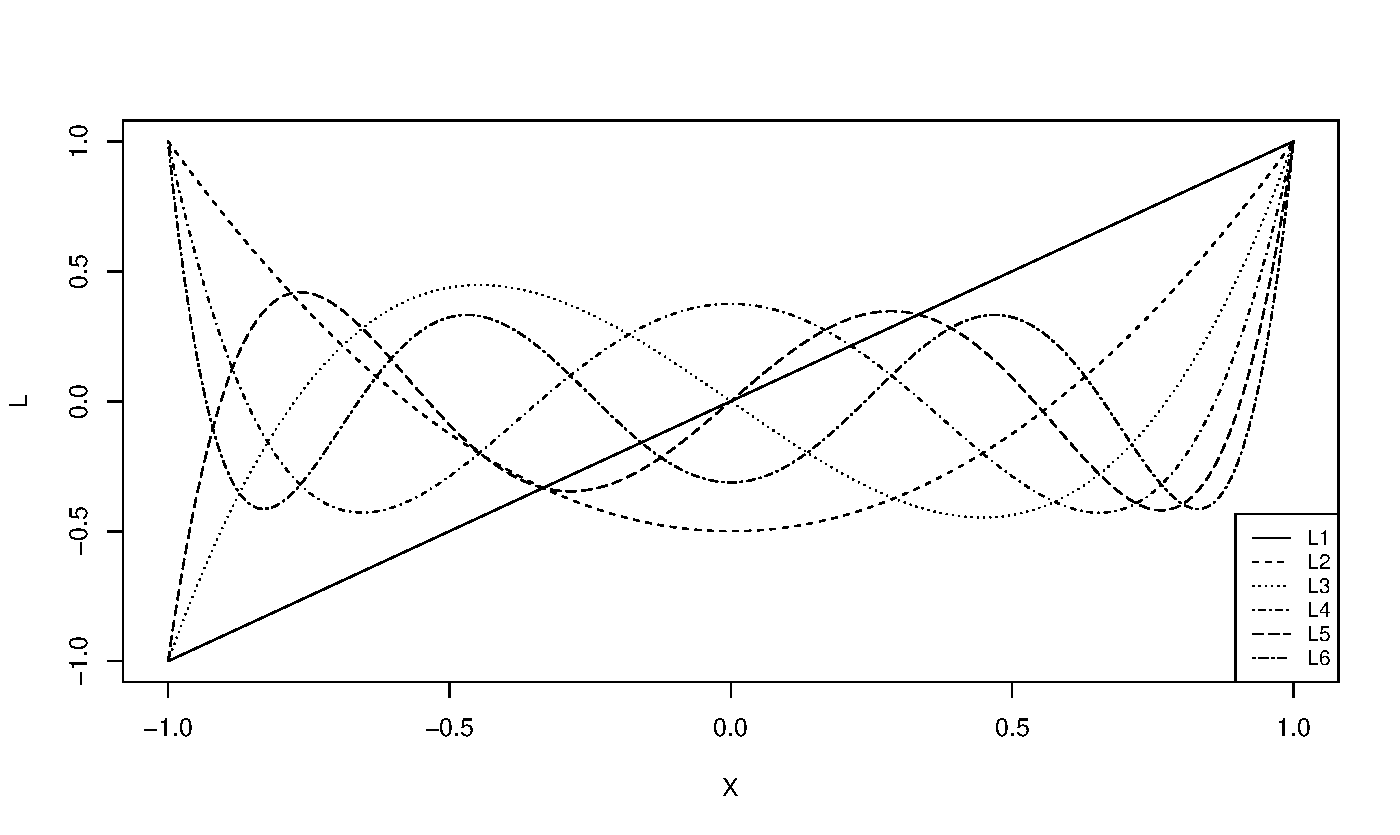
\includegraphics[width = 1.0\textwidth,trim= {{0\textwidth} {0\textwidth} {0\textwidth} {0.1\textwidth}}, clip=true] {Graphics/legendre.plot.pdf}
		%}
		\caption{The first six Legendre polynomial basis}
		\label{legendre_poly_plot}
	\end{figure}

        As is seen in Figure \ref{legendre_poly_plot}, range of the first six Legendre polynomials\footnote{Actually, range of all Legendre polynomials are bounded in $[-1,1]$.} are bounded in $[-1,1]$. However, sometimes if we hope to have orthonormal Legendre polynomials, we need to further nomalize them which may then make them unbounded in range. See more discussions in Appendix \ref{normalized_legendre}. 

        \subsubsection{Splines}\label{splines}

        In general, a spline is a piecewise polynomial, the order of which is pre-selected. The flexibility of splines lies in the number of polynomial segments. The joints between segments are called knots. To put it formally, a $(q+1)^{th}$ order\footnote{Accordingly, the degree of piecewise polynomial is $q$. Please be aware that degree=order-1.} spline with $N$ internal knots $\tau_1 < \tau_2 < \cdots < \tau_N$ has $N+q+1$ spline bases, and we can write them in vector notation.
        \begin{align}
            p^{K_n}(X)=p^{N_n+q+1}(X)=
            \begin{pmatrix}
                1  \\
                X  \\
                \vdots \\
                X^q\\
                (X-\tau_1)^q \mathds{1}\{X \ge \tau_1\}  \\
                \vdots  \\
                (X-\tau_{N_n})^q \mathds{1}\{X \ge \tau_{N_n}\}
            \end{pmatrix} 
        \end{align}

        where $K_n=N_n+q+1$. Since $K_n$ in sieve space grows slowly with $n$, the number of internal knots $N_n$ should also increase slowly with $n$ to ensure the consistency of sieve estimation. Moreover, in this thesis, once the number of internal knots $N_n$ is given, we define the positions of knots as quantiles $j/(N_n+1)$ for $j \in (1, \ldots, N_n)$ so that the probability mass is equalized across all segments. This rule of defining knot positions also applies to the construction of following B-Splines.

        \subsubsection{B-Splines}\label{b-splines}

        B-spline is short for basis spline, and B-splines of order $(q+1)$ are basis functions of splines with the same order over the same knots. All possible splines can be built from a linear combination of B-splines, and the linear combination is unique for each spline. In consistence with the definition of splines, let $N_n$ denote the number of internal knots, and let $q$ be the polynomial degree of spline. Then, in the construction of B-splines, we have a total number of knots $M_n=N_n+2\times(q+1)$ with $q+1$ overlapping knots at each boundary. Knots are indexed as $\tau_0 \le \tau_1 \le \cdots \le \tau_{M_n-1}$. The $i^{th}$ B-spline for a $(q+1)^{th}$ order spline could then be built by Cox-de Boor recursion formula.
        \begin{align} \label{b-splines_formula}
        \begin{split}
            B_{i,0}(X)& =
            \begin{cases}
                1 & \mathrm{if} \quad \tau_i \le X \le \tau_{i+1}\\
                0 & \mathrm{otherwise}
            \end{cases}\\
            B_{i,q}(X) &= \frac{X-\tau_i}{\tau_{i+q}-\tau_i}B_{i,q-1}(X)+\frac{\tau_{i+q+1}-X}{\tau_{i+q+1}-\tau_{i+1}}B_{i+1,q-1}(X)
        \end{split}
        \end{align}

        where $0 \le i \le M_n-1-q-1=N_n+q$. Obviously, we have $M_n-q-1=N_n+q+1$ B-splines for a $(q+1)^{th}$ order spline with $N_n$ internal knots. Figure \ref{bspline_plot} depicts B-Splines with polynomial degree $q=3$ and a total number of knots $M_n=11$ ($q+1=4$ overlapping knots at each boundary and $N_n=3$ internal knots) on $[0,1]$. 
        
        \begin{figure}[H]
		%\makebox[\textwidth][c]{
	    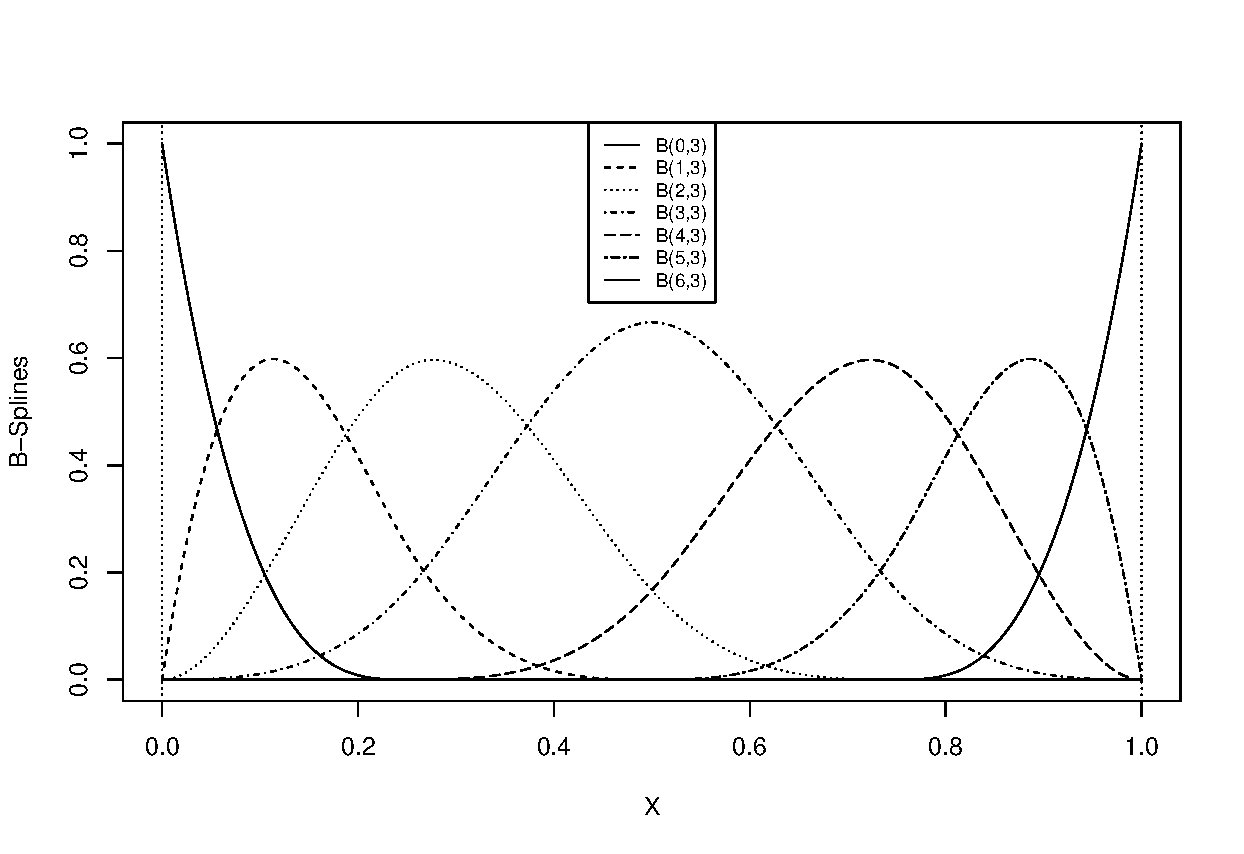
\includegraphics[width = 1.0\textwidth, trim= {{0\textwidth} {0\textwidth} {0\textwidth} {0.1\textwidth}}, clip=true] {Graphics/bspline.plot.pdf}
		%}
		\caption{B-splines}
		\label{bspline_plot}
	\end{figure}

        In Figure \ref{bspline_plot}, $B(i,q)$ correponds to $B_{i,q}$ in (\ref{b-splines_formula}). This set of seven B-Splines can be used to create any spline function with order of 4 (i.e., polynomial degree 3) and over the same knots\footnote{See \url{http://web.mit.edu/hyperbook/Patrikalakis-Maekawa-Cho/node17.html} for a similar example and more details about B-Splines.}. 

        \subsubsection{Trigonometric Polynomials}\label{trig_poly}

        For $X \in [-1,1]$, we can write trigonometric polynomial bases in a vector notation, using an $n$-varying $K_n$.
        \begin{align}
            p^{K_n}(X)=
            \begin{pmatrix}
                1  \\
                \cos(\pi X)  \\
                \sin(\pi X) \\
                \vdots \\
                \cos(K_n \pi X)  \\
                \sin(K_n \pi X) \\
            \end{pmatrix} 
        \end{align}

        Trigonometric polynomials are orthogonal in the domain of $[-1,1]$. See Appendix \ref{normalized_trig_poly} for the proof. They are a combination of sine and cosine polynomials, thus likely being good at approximating periodic functions.

        \subsubsection{Haar Wavelets}\label{haar_wavelets}

        Haar sequence was proposed by \cite{Haar_1910}, and later they were designed to be one of the most well-known wavelets. To construct Haar basis functions, original variables should be rescaled to $[0,1]$, and there is an increasing level in their construction. In level 0, there is only one basis function, and in level 1, there become two basis functions. With the level going up, the number of basis functions doubles. To put it formally, we denote level as $j \in \{0,1,2,\ldots\}$, so the number of basis functions in each level is $2^j$. Let $k \in \{0,1,\ldots, 2^j-1\}$ represent the index of basis functions in each level. For $X \in [0,1]$, the normalized and shifted Haar basis functions\footnote{In practice, there is usually an additional basis function which is equal to 1 over $X \in [0,1]$. It is used to approximate intercept.} are:
        \begin{align}
            \psi_{jk}(X)=2^{j/2}\psi(2^jX-k)
        \end{align}

        with
        \[
            \psi(X)=
            \begin{cases}
                1 & \mathrm{if} \quad 0 \le X < 1/2 \\
                -1 & \mathrm{if} \quad 1/2 \le X < 1 \\
                0 & \mathrm{otherwise}
            \end{cases}
        \]

        It is found that the basis function $\psi_{j,k}(X)$ is supported on a right-open interval $[\frac{k}{2^j}, \frac{k+1}{2^j})$ and it vanishes outside this interval. With some simple calculations, Haar basis functions are obviously pairwise orthogonal. Moreover, since Haar basis functions are normalized here, the $L_{\infty}$-norm is $||\psi_{jk}(X)||_{\infty}=2^{j/2}$, which increases with level exponentially. 
        
        \newpage
        \section{Lasso-type Methods}\label{lasso-type_method}

        In Section \ref{sieve}, we have clarified how to build up a finite-dimensional multivariate sieve space from original independent variables. Sieves are proven to have good approximation of unknown functions under certain assumptions (\cite{Chen_2007}). In this section, we will introduce two Lasso-type methods, which are then applied to select significant terms in the constructed sieve, thus realizing dimension reduction without losing prediction accuracy. These methods are employed in the second step of our dimension adaptive estimation, and are crucial in adapting the convergence rate of our estimator to underlying dimensionality of different true models.

        \subsection{Lasso}\label{lasso}

        The Lasso, proposed by \cite{Tibshirani_1996}, is short for \textit{Least Absolute Shrinkage and Selection Operator}. It is popular for high-dimensional problems due to its statistical accuracy of prediction and computationally feasible variable selection. \\

        Consider a setting where $(Z_1, Y_1), \ldots, (Z_n,Y_n)$ is a sample of independent random pairs $(Z,Y)$ with $Z \in \mathbb{R}^p$ being covariates and $Y \in \mathbb{R}$ being a response variable. For a continuous $Y$, a simple approach is to establish a linear model.
        \begin{align}\label{linear_model}
            Y=\sum\limits_{j=1}^p Z_j\beta_j+\epsilon
        \end{align}

        where $Z_j=(Z_{1j}, Z_{2j}, \ldots, Z_{nj})^{T}$ for $j=1,2,\ldots,p$, and $E[\epsilon|Z]=0$. A straightforward estimation method is Ordinary Least Squares (OLS). This would not be a problem if $p<n$. However, if $p>n$, OLS estimator is not unique any more and will heavily overfit the sample data. This is particularly true for our research when the number of terms in multivariate sieve space is usually much larger than the sample size. Therefore, a technique is needed to reduce complexity while maintaining approximation accuracy. Lasso is such a dimension reduction technique, and it does so with a regularization of $\ell_1$ penalty. The Lasso estimator for linear model in (\ref{linear_model}) is:
        \begin{align}\label{lasso_estimator}
            \hat{\beta}(\mathrm{lasso})=\arg\min\limits_{\beta} \left(\left|\left|Y-\sum\limits_{j=1}^p Z_j\beta_j\right|\right|^2+\lambda\sum\limits_{j=1}^p\left|\beta_j\right| \right)
        \end{align}

        where $\lambda$ is a non-negative regularization parameter. $||\cdot||^2$ indicates squared $L_2$ norm. The second term in (\ref{lasso_estimator}) is the so-call $\ell_1$ penalty, which is key to dimension reduction.\\
        
        Specifically, Lasso diminishes coefficients to 0 as $\lambda$ increases, because it has to balance the two terms in (\ref{lasso_estimator}) such that the summation is minimized. If $\lambda$ is sufficiently large, some coefficients are diminished to exact 0\footnote{The reason behind some coefficients being shrunk to exact 0 instead of extremely small values lies in the shape of $\ell_1$ constraint. See Page 9-19 of \cite{Bühlmann_van_de_Geer_2011} for details.}. The variables corresponding to those coefficients are usually of little significance to approximating the response variable, so their being exact 0 only sacrifices a little bit in-sample approximation accuracy but gains much in dimension reduction. Owing to such a bias-variance trade-off, Lasso often helps to improve out-of-sample prediction accuracy. Also, it has been discovered that $\ell_1$ regularization can find out the "right" sparse representation of underlying models with certain assumptions (\cite{Donoho_Elad_2003}). \\

        That being said, in using Lasso for prediction, there are still three more issues researchers need to be aware of. Firstly, variables need to be rescaled beforehand, because the rule of variable selection depends on the scale of coefficients, which is associated with the magnitude of variables. To remove such an unfair influence of magnitude, one needs to rescale variables before the use of Lasso\footnote{See Appendix \ref{standardization_of_lasso} for more details of why rescaling before analysis is required. Moreover, good news is that \href{https://glmnet.stanford.edu/}{glmnet}, the most popular R package for Lasso, implicitly does standardization inside the code by default, so usually there is no need to worry.}. Secondly, the regularization parameter $\lambda$ in (\ref{lasso_estimator}) is pre-defined, but researchers usually don't know how large it should be in practice. Thus, cross-validation is commonly applied to select the "best" $\lambda$ for Lasso. Thirdly, because $\ell_1$ regularization can recover the "right" sparsity of underlying models, we can always estimate the model very well simply by performing an OLS regression restricted to the selected subset (Section 11.4 of \cite{Hastie_Tibshirani_Wainwright_2015}). It is a common practice to run OLS (for a linear model) on all selected variables from Lasso, which is the so-called post Lasso Method\footnote{\cite{Belloni_Chernozhukov_Hansen_2013} argue that one needs to be cautious about doing inference with post Lasso due to the failure of uniform inference. They develop a "post-double-selection" method which is able to perform inference uniformly.}. The estimated coefficients from post Lasso can then be used for prediction on a test or new dataset.\\

        The concept of Lasso also extends to cases of generalized linear models including Logistic model and Poisson model. Please refer to Chapter 3 of \cite{Bühlmann_van_de_Geer_2011} for such extensions. Under these models, the estimation methods for post Lasso should also be changed from OLS to other methods accordingly. 

        \subsection{Adaptive Lasso}

        Despite the fact that Lasso has a good performance in dimension reduction, its consistency with respect to variable selection is not guaranteed unless some conditions are satisfied. \cite{Meinshausen_Bühlmann_2006} show a condition that such consistency of Lasso may need, and they claim that the condition can not be further relaxed. \cite{Zou_2006} also summarises and re-interprets this necessary condition, but he further asks himself if Lasso could be revised in a way such that the new estimator is still consistent even when that condition is further considerably relaxed. His answer is yes, and he terms the new estimation method as \textit{adaptive Lasso}.\\

        As shown in (\ref{lasso_estimator}), with a ubiquitous penalization parameter $\lambda$, Lasso forces all coefficients to be equally penalized. To revise it, \cite{Zou_2006} allows different weights to different coefficients, and adaptive Lasso is thus actually a weighted Lasso. Suppose $\hat{\beta}$ is a root-$n$ consistent estimator to the true parameter $\beta$. For example, it can be an OLS estimator. Pick up a tuning parameter $\gamma > 0$ (usually $\gamma=1$), and the weight for coefficient $\beta_j$ is defined as $\hat{w}_j=1/|\hat{\beta}_j|^{\gamma}$. Then, the adaptive lasso estimator for the linear model in (\ref{linear_model}) is given:
        \begin{align}\label{adaptive_lasso_estimator}
            \hat{\beta}(\mathrm{adaptive}\: \mathrm{lasso})=\arg\min\limits_{\beta} \left(\left|\left|Y-\sum\limits_{j=1}^p Z_j\beta_j\right|\right|^2+\lambda\sum\limits_{j=1}^p\hat{w}_j\left|\beta_j\right| \right)
        \end{align}

        In (\ref{adaptive_lasso_estimator}), it is seen that the penalization for larger coefficients is smaller, thus making them have a higher chance of survival in variable selection. \cite{Zou_2006} has proved that adaptive Lasso is consistent in variable selection with a much more relaxed condition than Lasso. he also clarifies that adaptive Lasso could be solved by the same efficient algorithm as that for solving Lasso. Moreover, the method of adaptive Lasso can easily be extended to generalized linear models as well.\\

        In practice, adaptive Lasso is often realized in a two-stage approach. Firstly, Lasso is performed on original dataset, so some variables are selected with non-zero coefficients. In order to obtain the estimated coefficients\footnote{Sometimes, estimated coefficients from Lasso or ridge regression are used to calculate weights even though they are not from a root-$n$ consistent estimator.} from a root-$n$ consistent estimator, post Lasso is usually applied on those selected variables. Secondly, estimated coefficients from post Lasso are applied to calculate weights which are then used in adaptive Lasso. \\

        Again, to get estimated coefficients for prediction in a test or new dataset, it is a usual practice to perform post adaptive Lasso just like how we do post Lasso, i.e., running OLS (for linear models) on selected terms from adaptive Lasso. 

        \newpage
        \section{\cite{Bunea_2007}} \label{bunea_paper}
            In this section, we introduce a major theorem established in \cite{Bunea_2007}, which will be later used to argue about the properties of our dimension adaptive estimator. In their paper, they show that Lasso-type estimator in random design non-parametric regression satisfies sparsity oracle inequalities\footnote{In a reference to \cite{Koltchinskii_2011}, "an oracle inequality is a bound on the risk of a statistical estimator that shows that the performance of the estimator is almost (often, up to numerical constants) as good as it would be if the statistician had an access to an oracle that knows what the best model for the target function is".}, i.e., bounds in terms of the number of non-zero components of the oracle vector. They prove that the finding holds even when the original dimension of data is much larger than the sample size or the regression matrix is not positive definite.\\
            
            This setting of random design non-parametric regression fits well into our research, because the first step of our dimension adaptive estimation is the generation of a multivariate sieve space from original dataset as shown in (\ref{sieve_space_multivariate}). This is a random design non-parametric technique where the number of terms in the generated sieve grows slowly with sample size. Therefore, the oracle inequalities established in their paper is crucial in arguing about the properties of our dimension adaptive estimation.\\

            Section \ref{setup} introduces the random design non-parametric setup in their paper, and Section \ref{sparsity_and_dimension_reduction} presents the concepts of sparsity and weak sparsity which are used in their theorem. In Section \ref{assumptions}, assumptions of the theorem are listed and Section \ref{sparsity_oracle_inequalities} concludes this chapter with their theorem that we will use later in Chapter \ref{dimension_adaptive_estimation}.
            
            \subsection{Setup}\label{setup}
                Let $(X_1, Y_1), \ldots, (X_n,Y_n)$ be a sample of independent random pairs with $(X,Y) \in (\mathcal{X},\mathbb{R})$, where $\mathcal{X}$ is a Borel subset of $\mathbb{R}^d$. Denote $\mu$ as the probability measure of $X$. Assume $g(X)=E(Y|X)$ to be the unknown conditional mean function and $\mathcal{G}_M=\{g_1, \ldots,g_M\}$ to be a finite dictionary of real-valued functions $g_j$ that are defined on $\mathcal{X}$. For example, $\mathcal{G}_M$ can be a collection of basis functions used to approximate $g$ in series estimation\footnote{More specifically, with a relation to our own research, $\mathcal{G}_M$ can be seen as a collection of all terms in the multivariate sieve space we have created in (\ref{sieve_space_multivariate}), because those product-terms can also be viewed as basis functions for interactions among different variables. So, $M$, the length of dictionary, would then be $(K_n+1)^d$ in our own research.}. Then, for any $\beta=(\beta_1,\ldots,\beta_M) \in \mathbb{R}^M$, the penalized least squares (i.e., Lasso-type) estimator is:
                \begin{align}\label{lasso-type_estimator}
                    \widehat{\beta}=\arg\min_{\beta \in \mathbb{R}^M}\left\{ \frac{1}{n} \sum\limits_{i=1}^n \{Y_i-g_{\beta}(X_i)\}^2+2\sum_{j=1}^M \omega_{n,j}|\beta_j| \right\}
                \end{align}

                where $g_{\beta}(x)=\sum_{j=1}^M\beta_jg_j(x)$, $\omega_{n,j}=r_{n,M}||g_j||_n$ and $||g_j||_n$ is the empirical $L_2$ norm of function $g_j$. The choice of tuning sequence $r_{n,M}>0$ will be discussed in Section \ref{sparsity_and_dimension_reduction}. Consequently, $\widehat{g}=\sum_{j=1}^M \widehat{\lambda}_jg_j$ is an estimate of $g$. Despite the fact that oracle properties of such a Lasso-type estimator have been well studied in linear parametric regression and fixed design non-parametric regression where $M$ is fixed and $n \to \infty$, its oracle properties in random design non-parametric regression have only received little attention. To bridge this gap, \cite{Bunea_2007} tries to establish oracle inequalities for the approximation error $||\widehat{g}-g||^2$ and the $\ell_1$-loss $|\widehat{\beta}-\beta|_1$ in a random design non-parametric setting where $M=M(n)$ and possibly much larger than $n$.

            \subsection{Sparsity and Dimension Reduction}\label{sparsity_and_dimension_reduction}
                To introduce the concept of sparsity, let us consider a linear regression at first. The OLS estimator $\widehat{\beta}_{OLS}$ for the linear regression is almost the same as $\widehat{\beta}$ defined in (\ref{lasso-type_estimator}) but without a penalty term. Obviously, the $\ell_1$-loss $|\widehat{\beta}_{OLS}-\beta|_1$ is of order $M/\sqrt{n}$ in probability if $\widehat{\beta}$ is based on all $M$ regressors, then the estimation error can be very large in case of high dimensionality (large $M$). This gives rise to the concept of sparsity.

                \begin{definition}[Sparsity]\label{sparsity}
                    Let $M(\beta)$ denote the number of non-zero coefficients of $\beta$, then
                    \begin{align}
                        M(\beta)=\sum\limits_{j=1}^M \mathds{I}_{\{\beta_j \not= 0\}}=\mathrm{Card} J(\beta)
                    \end{align}

                    where $\mathds{I}_{\{\cdot\}}$ is indicator function and $J(\beta)=\{j \in \{1, \ldots, M\}: \beta_j \not=0\}$. 
                \end{definition}

                The smaller $M(\beta)$, the sparser $\beta$. By taking advantage of sparsity, their paper shows that the $\ell_1$-loss of lasso-type estimator $\widehat{\beta}$, i.e., $|\widehat{\beta}-\beta|_1$ is bounded, up to known constants and logarithms, by $M(\beta)/\sqrt{n}$, if in the penalty term, we have $r_{n,M}=A\sqrt{(\log M)/n}$ where $A$ is a sufficient large constant. That means, the estimation error will be much smaller if $\beta$ is much sparser.\\

                It is worthy of mentioning that in Setup \ref{setup}, $g_{\beta}$ is not an exact representation of $g$, but a series approximation instead. Thus, the concept of sparsity in Definition \ref{sparsity} is too strong for this setup. Therefore, \cite{Bunea_2007} introduce weak sparsity.

                \begin{definition}[Weak Sparsity]\label{weak_sparsity}
                    Let $C_g >0$ be a constant depending on $g$, and denote 
                    \begin{align}
                    \mathcal{B}=\{\beta \in \mathbb{R}^M: ||g_{\beta}-g||^2 \le C_g r_{n,M}^2 M(\beta)\}
                    \end{align}
                    as the oracle set. Here, $||\cdot||$ is the $L_2(\mu)$-norm with probability measure $\mu$, and $\langle f,g\rangle$ denotes the corresponding scalar product for any $f,g \in L_2(\mu)$. Then, if $\mathcal{B}$ is non-empty, $g$ is said to have a weak sparsity property relative to the dictionary $\mathcal{G}_M=\{g_1,\ldots,g_M\}$.
                \end{definition}

                With the definition of weak sparsity, one may have the belief that, for some $\beta^* \in \mathbb{R}^M$, the squared approximation error $||g_{\beta^*}-g||^2$ is bounded, up to logarithmic factors, by $M(\beta^*)/n$. The order of this approximation error is much smaller than the one without dimension reduction. Similar to the oracle vector $\beta$ in case of linear regression, $\beta^*$ is the oracle vector in this case of series approximation, and it is defined as:
                \begin{align}
                    \beta^*=\arg\min\{ ||g_{\beta}-g||:\beta \in \mathbb{R}^M, M(\beta)=k^* \}
                \end{align}

                where $k^*=\min\{ M(\beta):\beta \in \mathcal{B}\}$ is called oracle dimension. 

            \subsection{Assumptions}\label{assumptions}
            The authors explicitly make three assumptions, which are necessary for their theorem to hold. Following the notation in Setup \ref{setup}, the error terms are defined to be $W_i=Y_i-g(X_i)$. Also, recall $g(X)=E(Y|X)$ is the unknown conditional mean function.
            \begin{assumption}\label{assumption_1}
                $X_1, \ldots, X_n$ are independent, identically distributed random variables with probability measure $\mu$. Random variables $W_i$ are independently distributed with $E\{W_i|X_1,\ldots,X_n\}=0$ and $E\{\exp(|W_i|)|X_1,\ldots,X_n\}\le b$ for some finite $b>0$ and $i=1,\ldots,n$.
            \end{assumption}

            This is a standard assumption to ensure the statistical properties of an estimator. Zero conditional mean of $W_i$ ensures the linear independence between $W_i$ and $X$, so the expectation of $W_i$ does not change with the values of $X$. Meanwhile, $E\{\exp(|W_i|)|X_1,\ldots,X_n\}\le b$ guarantees the existence of moments for error terms.

            \begin{assumption}\label{assumption_2}
                Define $||h||_{\infty}=\sup_{x \in \mathcal{X}}|h(x)|$ as sup norm for any bounded function $h$ on $\mathcal{X}$.
                \begin{enumerate}[label=(\alph*), noitemsep]
                    \item There exists $0<L<\infty$ such that $||g_j||_{\infty} \le L$ for all $1 \le j \le M$.
                    \item There exists $c_0 >0$ such that $||g_j||\ge c_0$ for all $1 \le j \le M$.
                    \item There exists $L_0 < \infty$ such that $E[g_i^2(X)g_j^2(X)] \le L_0$ for all $1 \le i,j \le M$.
                    \item There exists $L_* < \infty$ such that $||g||_{\infty} \le L_* < \infty$.
                \end{enumerate}
            \end{assumption}

            This assumption imposes mild conditions on $g$ and basis functions $g_j$, which are in the dictionary $\mathcal{G}_M$. It is noted that (a) implies (c) trivially. But, as $L$ in (a) might be too large, they state (c) separately. The implication of (a) and (d) is that for any fixed $\beta \in \mathbb{R}^M$, there exists a positive constant $L(\beta)$, such that $||g-g_{\beta}||_{\infty}=L(\beta)$.

            \begin{assumption}\label{assumption_3}
                For any $M \ge 2$, there exist constants $\kappa_M>0$ such that $\Psi_M-\kappa_M\mathrm{diag}(\Psi_M)$ is positive semi-definite, where $\Psi_M$ is a $M \times M$ matrix given by
                \begin{align}\label{psi_m}
                    \Psi_M=(E g_j(X)g_{j^{\prime}}(X))_{1 \le j,j^{\prime} \le M}=\left( \int g_j(x)g_{j^{\prime}(x)}\mu(dx) \right)_{1 \le j, j^{\prime} \le M}
                \end{align}
            \end{assumption}

            Due to the positive semi-definiteness of $\Psi_M-\kappa_M\mathrm{diag}(\Psi_M)$, they note that $0< \kappa_M \le 1$. Along with part (b) of Assumption (\ref{assumption_2}), Assumption (\ref{assumption_3}) implies that $\Psi_M$ is positive definite, with the minimal eigenvalue $\tau$ bounded below by $c_0\kappa_M$. 
            
            \subsection{Theorem of Sparsity Oracle Inequalities}\label{sparsity_oracle_inequalities}

            With assumptions (\ref{assumption_1}) - (\ref{assumption_3}), the authors have proved the sparsity oracle inequalities for the lasso-type estimator $\widehat{\beta}$, as defined in (\ref{lasso-type_estimator}).

            \begin{theorem}\label{oracle_inequalities_theorem}
                Assume that Assumptions (\ref{assumption_1}) - (\ref{assumption_3}) hold. Then, for all $\beta \in \mathcal{B}$ we have
                \begin{align}
                    &\mathbb{P}\left\{ ||\widehat{g}-g||^2 \le B_1 \kappa_M^{-1} r_{n,M}^2 M(\beta) \right\} \ge  1-\pi_{n,M}(\beta)\\
                    &\mathbb{P}\left\{ |\widehat{\beta}-\beta|_1 \le B_2 \kappa_M^{-1} r_{n,M} M(\beta) \right\} \ge 1-\pi_{n,M}(\beta)
                \end{align}
                where $B_1>0$ and $B_2>0$ are constants depending on $c_0$ and $C_g$ only and
                \begin{align}\label{pi_n_M}
                \begin{split}
                    \pi_{n,M}(\beta) \le & 10M^2 \exp\left( -c_1n \min \left\{ r_{n,M}^2, \frac{r_{n,M}}{L}, \frac{1}{L^2}, \frac{\kappa_M^2}{L_0 M^2(\beta)}, \frac{\kappa_M}{L^2M(\beta)} \right\} \right)\\
                    & +\exp\left( -c_2 \frac{M(\beta)}{L^2(\beta)}nr_{n,M}^2 \right)
                \end{split}
                \end{align}
                for some positive constants $c_1$, $c_2$ depending on $c_0$, $C_g$ and $b$ only and $L(\beta)=||g-g_{\beta}||_{\infty}$.
            \end{theorem}

            This theorem is very useful in the case of weak sparsity. By replacing $\beta$ and $M(\beta)$ with $\beta^*$ and $M(\beta^*)$ which are defined at the end of Section \ref{sparsity_and_dimension_reduction}, Theorem \ref{oracle_inequalities_theorem} indicates that, under some assumptions, the squared approximation error of lasso-type estimator is controlled, up to a logarithmic factor, by a bound that only relates to the number of non-zero components of oracle vector, instead of all components. In other words, the sparser the oracle vector is, the smaller the squared error and the faster the convergence rate will be. This is conducive to the dimension adaptive properties of our estimator in Section \ref{dimension_adaptive_estimation}.

        \newpage
        \section{Dimension Adaptive Estimation}\label{dimension_adaptive_estimation}
            In this section, we will apply Theorem \ref{oracle_inequalities_theorem} to show that a combination of sieve estimation and Lasso-type methods leads to an estimator, the convergence rate of which can adapt to the dimensionality of underlying true model, up to a logarithmic factor. \\

            Section \ref{estimation_steps} restates and summarizes the steps of our dimension adaptive estimation, and in Section \ref{underlying_models}, we list three different types of underlying true models, on which we hope to examine the properties of our dimension adaptive estimation. Section \ref{dae_assumptions} tailors assumptions (\ref{assumption_1}) - (\ref{assumption_3}) to fit the underlying models we consider. Section \ref{oracle_properties} closes this chapter with a theorem on the convergence rate of our dimension adaptive estimation.

            \subsection{Estimation Steps}\label{estimation_steps}
                There are generally two steps in dimension adaptive estimation. The first step is to construct a multivariate sieve space from the original group of independent variables by using a specific type of basis functions, with reference to (\ref{sieve_space_multivariate}). The total number of terms in the sieve should grow slowly with sample size to ensure consistency of sieve estimation, and in Section \ref{underlying_models}, we will discuss how it changes with sample size. \\
                
                The second step is to apply Lasso-type methods as discussed in Chapter \ref{lasso-type_method} to select significant terms in the constructed sieve, thus achieving dimension reduction without losing prediction accuracy. The Lasso-type methods are essential in finding the oracle dimension in underlying models. If a researcher hopes to make prediction on a new dataset, it is recommended to get estimated coefficients from running OLS (for linear models) on selected terms of Lasso-type methods, and use those coefficients for prediction. 

            \subsection{Three Underlying Models}\label{underlying_models}
                Let $(X_1, Y_1), \ldots, (X_n,Y_n)$ be a sample of independent random pairs with $(X,Y) \in (\mathcal{X},\mathbb{R})$, where $\mathcal{X}$ is a Borel subset of $\mathbb{R}^d$. Here, $X$ is normalized such that $X_d \in [0,1]$ for all $d \in \{1,2,\ldots\}$ . Consider the following model:
                \begin{align}
                    Y=g(X)+W, \quad E(W|X)=0
                \end{align}
                where $W$ is the error term with zero conditional mean, then $E(Y|X)=g(X)$ is the unknown conditional mean function. Suppose $g(X)$ to be a $p$-smooth function with $s$-times continuous derivatives as defined in \ref{p-smooth_function}. \\

                Let $\{p_k(\cdot)\}_{k=0}^{\infty}$ be basis functions for each dimension of $X$, i.e., each regressor. Then, we consider the product-terms $\{\prod_{l=1}^{d}p_{k_l}(x_l)\}_{k_l=0}^{\infty}$ to be basis functions for interactions among different regressors. In this thesis, we consider three different underlying models. In model (a) and (b), we are dealing with a non-parametric model with infinite dimension, while in model (c), parametric model with finite dimension. Hopefully, our estimator can successfully adapt its convergence rate to all three types of underlying true models.

                \subsubsection{Model (a): Unrestricted Underlying Model}\label{unrestricted_model}
                
                In this model, unknown parameters are assumed to lie in infinite-dimensional parameter spaces, so it would be computationally difficult to estimate such a model by using finite samples. Instead, we use sieve estimation, specifically series estimation. But to ensure consistency, the complexity of sieves should increase with the sample size so the number of basis functions for each regressor, $K_n$, grows slowly with sample size $n$. To put it formally, suppose there is a positive constant $s$ and $\beta \in \mathbb{R}^{(K_n+1)^d}$ such that
                \begin{align}
                     \sup_{x \in \mathcal{X}} \left| g(x) - \sum_{k_1=0}^{K_n} \cdots \sum_{k_d=0}^{K_n} \beta_{k_1,\ldots,k_d}\prod_{l=1}^{d}p_{k_l}(x_l) \right|=\mathcal{O}(K_n^{-s})
                \end{align}
                Sufficient conditions for this supremum consistency has been briefly discussed in Section \ref{sieve_extremum_estimation}, or one can refer to Chapter 3 of \cite{Chen_2007}. From the above supremum norm of approximation bias, it is easy to show that the squared bias of series estimator is of order $K_n^{-2s}$. The variance of series estimator is of order $K_n^d/n$, as shown in \cite{Newey_1997}. \\
                
                The orders of both squared bias and variance involve $K_n$. It implies that the growth of $K_n$ will reduce the squared bias but also increase variance. It is important to find a trade-off between them so that the optimal rate of $K_n$ is achieved. In other words, we can choose $K_n$ such that
                \begin{align*}
                    K_n^{-2s} \asymp \frac{K_n^d}{n}  \Leftrightarrow  K_n \asymp n^{\frac{1}{2s+d}}
                \end{align*}

                Therefore, $(K_n+1)^d$, the number of non-zero coefficients in model (a), is of order $n^{\frac{d}{2s+d}}$.

                \subsubsection{Model (b): Additive Underlying Model}\label{additive_model}

                In this model, unknown parameters are still assumed to be in infinite-dimensional spaces but with an additional assumption of additivity\footnote{It implies no interactions between different regressors}. To ensure consistency, $K_n$ still grows slowly with $n$. To put it formally \footnote{Or, we can also use the formal representation from model (a), but with an additional restriction that $\sum_{l=1}^{d} \mathds{I}_\{k_l\not=0\}=1$ or $0$, where $\mathds{I}_{\{\cdot\}}$ is indicator function.}, suppose there is a positive constant $s$ and $\beta_1, \ldots, \beta_d \in \mathbb{R}^{K_n+1}$ such that
                \begin{align}
                    \sup_{x \in \mathcal{X}} \left| g(x) - \sum_{l=1}^{d} \sum_{k=0}^{K_n} \beta_{lk}p_k(x_l) \right|=\mathcal{O}(K_n^{-s})
                \end{align}

                Sufficient conditions for the supremum consistency can be found in Chapter 3 of \cite{Chen_2007}. It is easy to find that the squared bias is of order $K_n^{-2s}$, while the variance is of order $dK_n/n$, as proven in \cite{Newey_1997}. By following similar arguments as in model (a), we should choose $K_n$ such that 
                \begin{align*}
                    K_n^{-2s} \asymp \frac{dK_n}{n}  \Leftrightarrow  K_n \asymp n^{\frac{1}{2s+1}}
                \end{align*}
                
                Therefore, $d(K_n+1)$, the number of non-zero coefficient in model (b), is of order $n^{\frac{1}{2s+1}}$. 

                \subsubsection{Model (c): Parametric Underlying Model}\label{parametric_model}

                In this model, unknown parameters are assumed to lie in a finite-dimensional space. By Stone-Weierstrass Theorem (\cite{Stone_1948}), we know that the unknown function $g(X)$ can be uniformly approximated by basis functions. To put it formally, suppose there is $\beta \in \mathbb{R}^{(K+1)^d}$ for some fixed $K$\footnote{The fixed $K$ for different regressors can be varied. It doesn't make a change to our analysis.} such that
                \begin{align}
                    \sup_{x \in \mathcal{X}} \left| g(x) - \sum_{k_1=0}^{K} \cdots \sum_{k_d=0}^{K} \beta_{k_1,\ldots,k_d}\prod_{l=1}^{d}p_{k_l}(x_l) \right|=0
                \end{align}
                That is, we are dealing with a flexible parametric model. $K$ is finite and irrelevant to the sample size $n$. Apparently, the most usual parametric linear model falls into model (c).

                \subsection{Assumptions}\label{dae_assumptions}

                    In order to apply Theorem \ref{oracle_inequalities_theorem}, we need to tailor assumptions (\ref{assumption_1}) - (\ref{assumption_3}) proposed in Section \ref{assumptions} to fit into the setting of our own underlying models.\\

                    Please be aware that the use of different basis functions may lead to different valuation of parameters (e.g., $L$, $c_0$, $L_0$ and $\Psi_M$) in assumptions. To make our statements more consolidated over different basis functions, we orthonormalize them before the theoretical analysis, no matter which basis function we use\footnote{If we use Legendre and trigonometric polynomials as basis functions, we rescale the domain of $X_d$ to be $[-1,1]$ for its good property of orthogonality within this domain.}. How those parameters may change if we don't orthonormalize them beforehand is briefly discussed at the end of Appendix \ref{proof_of_corollary}.

                    \begin{assumption}\label{dae_assumption_1}
                        In accordance to Assumption (\ref{assumption_1}), we assume:
                        \begin{enumerate}[label=(\alph*), noitemsep]
                            \item $\{(X_i, Y_i)\}_{i=1}^n$ is a sample of independent random pairs with zero conditional mean of error terms, i.e., $E(W|X)=0$.
                            \item $E(\exp(|W|)|X)\le C_w$ for some constant $C_w>0$.
                            \item $g$ is a Hölder ($p$-smooth) continuous function and its smoothness, $s$, is bounded below by $\underline{s}$, that is, $s \ge \underline{s}$. 
                            \item $g$ is a bounded function on $\mathcal{X}$.
                            \item There exists a constant $C>0$ such that $||\prod_{l=1}^d p_{k_l}|| \le C$.
                        \end{enumerate}

                        Notice that, in the additive underlying model, $K_n$ is of order $n^{\frac{1}{2s+1}}$. Thus, for the unknown function $g$ with smoothness $s \ge \underline{s}$, the largest sieve space we use can be a linear span of basis functions up to an index sum of $C_sn^{\frac{1}{2\underline{s}+1}}$ with $C_s$ being sufficiently large (e.g., $C_s=\log(n)$). This sieve space would contain the best approximation in additive underlying model. That is,
                        \begin{align} \label{set_of_basis_function}
                            \prod_{l=1}^{d}p_{k_l}(x_l): \quad \sum_{l=1}^{d}k_l \le C_sn^{\frac{1}{2\underline{s}+1}}
                        \end{align}

                        Analogously, in unrestricted underlying model, the largest sieve space is a linear span of basis functions up to an index sum of $C_sn^{\frac{1}{2\underline{s}+d}}$ for $C_s$ large enough. This upper bound is smaller than that of additive model with $d \ge 2$, therefore $C_sn^{\frac{1}{2\underline{s}+1}}$ could also be used as an upper bound for the unrestricted model. Likewise, this sieve space also contains the best approximation for parametric model because $K$ is fixed. As a consequence, in the language of \cite{Bunea_2007}, we then have $M \lesssim n^{\frac{1}{2\underline{s}+1}}$.
                    \end{assumption}

                    \begin{assumption}\label{dae_assumption_2}
                        In accordance to Assumption (\ref{assumption_2}), we need to impose mild conditions on $g$ and on basis functions.
                        \begin{enumerate}[label=(\alph*), noitemsep]
                            \item There exists $0<L<\infty$ such that $||\prod_{l=1}^d p_{k_l}||_{\infty} \le L$ for all basis functions. 
                            \item There exists $c_0 >0$ such that $||\prod_{l=1}^d p_{k_l}|| \ge c_0$ for all basis functions. Since our basis functions are orthonormal, $c_0=1/C$ with $C$ from (e) of Assumption (\ref{dae_assumption_1}).
                            \item From (a) and (b), we have
                            \begin{align*}
                                E\left[\prod_{l=1}^d p_{k_l}^2(x_l)\prod_{l=1}^d p_{j_l}^2(x_l)\right] \le L^2E\left[\prod_{l=1}^d p_{k_l}^2(x_l)\right] \le L^2C_l\left|\left|\prod_{l=1}^d p_{k_l}(x_l)\right|\right|^2
                            \end{align*}
                            where $C_l$ is a positive constant. The first inequality comes from $||\prod_{l=1}^d p_{k_l}||_{\infty} \le L$. Due to the orthonormality of basis functions, we have $E\left[\prod_{l=1}^d p_{k_l}^2(x_l)\prod_{l=1}^d p_{j_l}^2(x_l)\right] \le L_0$ with $L_0=L^2$, ignoring the constant $C_l$.
                            \item By assumption, $g$ is a bounded function on $\mathcal{X}$, so $L^{*}$ is obviously bounded above.
                        \end{enumerate}
                    \end{assumption}
                    
                    \begin{assumption}\label{dae_assumption_3}
                         To save notation, let $g_k(X)=\prod_{l=1}^d p_{k_l}(x_l)$ denote basis functions with $1 \le k \le M$, and $g^M(X)=(g_1(X), \ldots, g_M(X))^T$ is then the vector of all basis functions. Accordingly, $\Psi_M=E[g^M(X)g^M(X)^{T}]$ in our setting. In accordance to Assumption (\ref{assumption_3}), for any $M \ge 2$, there exist constants $\kappa_M>0$ such that $\Psi_M-\kappa_M\mathrm{diag}(\Psi_M)$ is positive semi-definite. In fact, due to the orthonormality of basis functions we use, such a $\kappa_M$ exists and equal to $1/C^2$, which is bounded away from 0. See Appendix \ref{derivation_kappa} for proof.
                    \end{assumption}
                
                \subsection{Oracle Properties}\label{oracle_properties}
                    \subsubsection{Convergence Rates}\label{convergence_rates}
                    With assumptions (\ref{dae_assumption_1})-(\ref{dae_assumption_3}), Theorem \ref{oracle_inequalities_theorem} is then applied to obtain the optimal convergence rate of our estimator across all three underlying models we discuss in Section \ref{underlying_models}. \\

                    In Theorem \ref{oracle_inequalities_theorem}, ignoring constants, the squared $L_2$ norm of Lasso-type estimator, $||\hat{g}-g||^2$ is of order $r_{m,M}^2 M(\beta)$, as long as $\pi_{n,M}(\beta)$ is asymptotically zero. 

                    \begin{enumerate}[label=(\alph*), noitemsep]
                        \item In unrestricted underlying model, the number of non-zero coefficients $(K_n+1)^d$ is of order $n^{\frac{d}{2s+d}}$. In the language of \cite{Bunea_2007}, $M(\beta)=C_sn^{\frac{d}{2s+d}}$. Also, as suggested in Definition \ref{sparsity}, $r_{n,M}=A\sqrt{(\log M)/n}$. Then,
                        \begin{align*}
                            r_{n,M}^2M(\beta)= A^2 \frac{\log M}{n} C_sn^{\frac{d}{2s+d}} = A^2C_s \log M n^{-\frac{2s}{2s+d}}
                        \end{align*}
                        Hence, the optimal convergence rate of our estimator is $n^{-\frac{2s}{2s+d}}$, up to a logarithmic factor, in unrestricted underlying model.

                        \item In additive underlying model, the number of non-zero coefficients $d(K_n+1)$ is of order $dn^{\frac{1}{2s+1}}$ with $d$ being a constant. That means, $M(\beta)=C_sn^{\frac{1}{2s+1}}$. Then, 
                        \begin{align*}
                            r_{n,M}^2M(\beta)=A^2 \frac{\log M}{n}C_sn^{\frac{1}{2s+1}}=A^2 C_s \log M n^{-\frac{2s}{2s+1}}
                        \end{align*}
                        Hence, the optimal convergence rate of our estimator is $n^{-\frac{2s}{2s+1}}$, up to a logarithmic factor, in additive underlying model. 

                        \item In parametric underlying model, the number of non-zero coefficients is $(K+1)^d$, which is finite. That means, $M(\lambda)=(K+1)^d$. Then,
                        \begin{align*}
                            r_{n,M}^2M(\beta)=A^2 \frac{\log M}{n}(K+1)^d=A^2(K+1)^d\log M n^{-1}
                        \end{align*}
                        Hence, the optimal convergence rate of our estimator is $n^{-1}$, up to a logarithmic factor, in parametric underlying model. 
                    \end{enumerate}

                    To summarize, the theorem on convergence rate of our estimator is given as follows.
                    \begin{theorem}\label{convergence_rates_theorem}
                        Suppose that Assumptions (\ref{dae_assumption_1}) - (\ref{dae_assumption_3}) hold, and $\pi_{n,M}(\beta)$ in (\ref{pi_n_M}) is asymptotically zero. Then, the convergence rate of our estimator in squared $L_2$ norm is dimension adaptive with respect to underlying true models. Specifically, in unrestricted underlying model (\ref{unrestricted_model}), it converges at an optimal rate of $n^{-\frac{2s}{2s+d}}$; in additive model (\ref{additive_model}), $n^{-\frac{2s}{2s+1}}$; and in parametric model (\ref{parametric_model}), $n^{-1}$. All convergence rates are up to a logarithmic factor. 
                    \end{theorem}

                    It is seen that our dimension adaptive estimator can achieve an optimal convergence rate, regardless of the underlying true models, as if it were an "oracle" estimator. It converges in all three underlying models, even though with a different rate. Specifically, It converges as fast as a parametric estimator in parametric underlying model. In additive underlying model, the convergence rate is slower, and in unrestricted underlying model, it has the slowest convergence rate. In the latter two models, a parametric estimator will not convergence in probability to the true function.

                    \subsubsection{Lower Bound of Smoothness}\label{lower_bound_smoothness}
                    Theorem \ref{convergence_rates_theorem} holds true only if $\pi_{n,M}(\beta)$ defined in (\ref{pi_n_M}) is asymptotically zero. It is noted that $\pi_{n,M}(\beta)$ is related to parameters $L$ and $L_0$ which may change with the basis functions we use. For example, for unbounded basis functions, $L$ and $L_0$ might increase with sample size $n$ at some rate related to smoothness $s$, while for bounded basis functions, $L$ and $L_0$ are constants, irrelevant to $n$. Moreover, $M(\beta)$ in the inequality of $\pi_{n,M}(\beta)$ also relates to sample size $n$ and smoothness $s$. \\
                    
                    Therefore, the constraint on $\pi_{n,M}(\beta)$ will finally lead to a constraint on the lower bound of smoothness, and this lower bound is different for different basis functions. We thus have the following corollary, and see Appendix \ref{proof_of_corollary} for proof.
                    \begin{corollary}\label{smoothness_corollary}
                        Theorem \ref{convergence_rates_theorem} holds true only if the smoothness $s$ of the unknown regression function is bounded below by $\underline{s}$. This lower bound varies among different basis functions that we use to generate sieve for our dimension adaptive estimation. 
                        \begin{enumerate}[label=(\alph*), noitemsep]
                            \item For normalized Legendre polynomials, $\underline{s} > \frac{(2d-1)+\sqrt{8d^2+1}}{4}$, or a sufficient condition $\underline{s} \ge \frac{3d-1}{2}$.
                            \item For orthonormalized B-splines, $\underline{s}>\frac{d}{2}$, or a sufficient condition $\underline{s}\ge \frac{d+1}{2}$.
                            \item For normalized Haar wavelets, the same as (a).
                            \item For normalized trigonometric polynomials, same as (b).   
                            %constraint on $\pi_{n,M}(\beta)$ would always fail.
                        \end{enumerate}
                    \end{corollary}

                    As is mentioned in Section \ref{dae_assumptions}, to make our statement more consolidated, all basis functions are orthonormalized before analysis. Otherwise, their boundedness may change. Legendre polynomials, Haar wavelets and trigonometric polynomials on a specific domain are orthogonal by design, so a further normalization is enough. From Corollary \ref{smoothness_corollary}, it is seen that the lower bound of smoothness is more relaxed for orthonormalized B-splines and normalized trigonometric polynomials than the others. \\
                    %Whilst, the constraint on $\pi_{n,M}(\beta)$ doesn't hold if we use normalized Haar wavelets as basis functions, thus leading to failure of oracle property.\\

                    It is worthy of mentioning that the result in Corollary \ref{smoothness_corollary} is asymptotic. Even though the lower bound of smoothness for orthonormalized B-splines and normalized trigonometric polynomials are much more relaxed, it doesn't mean that they always outperform normalized Legendre polynomials and normalized Haar wavelets in finite samples. 
                    
        \newpage
        \section{Simulation Study}\label{simulation_study}
            \subsection{Simulation Setup}\label{simulation_setup}
                To illustrate how our dimension adaptive estimator behaves in finite samples, we apply it to simulated data and compare the results with "oracle" estimators that already know the dimensionality of underlying true models. According to the three types of underlying models discussed in Section \ref{underlying_models}, the following three functions are used in the illustrative simulated settings.
                \begin{align*}
                    m_1(x)=&3x_1+1.8x_2+x_3+2.5x_4+x_5 &\quad (x \in [0,1]^5)\\
                    m_2(x)=&\sin(4x_1)+1.5\log(x_2)+\frac{1}{\cos(x_3)}+\sin(\sqrt{x_4})+\sin(x_5^2) &\quad (x \in [0,1]^5)\\
                    m_3(x)=&3\sqrt[4]{x_1+4x_2+x_3x_4x_5}+2\sin(x_4+x_5^2+x_1x_2x_3)+3\log(x_3^2+x_4+2x_5) &\quad (x \in [0,1]^5)
                \end{align*}

                Among these functions, $m_1$ represents a parametric underlying model; $m_2$, an additive non-parametric model and $m_3$, an unrestricted non-parametric model. As shown in Theorem \ref{convergence_rates_theorem}, the dimension adaptive estimator can adapt its convergence rate to the unknown dimension of underlying model. That is, in model $m_1$, this estimator should converge as fast as a parametric estimator; in $m_2$, it should then be as good as a non-parametric estimator with additivity restriction; finally in $m_3$, it should outperform the other two estimators. \\

                In our simulation, the dimension adaptive estimator ($dimada$) is the sieve estimator with Lasso-type regularization as defined in Section \ref{estimation_steps}, and the non-parametric estimator with additivity restriction ($addt$) is an additive dimension adaptive estimator. The parametric estimator is just an ordinary least squares ($ols$) linear estimator.\\

                The $n$ observations of type $(X,Y)$ are generated with the following data generation process:
                \begin{align*}
                    Y=m_i(X)+\sigma_j \cdot \epsilon \quad \quad (i \in \{1,2,3\}, j \in \{1,2\})
                \end{align*}

                where $X$ is uniformly distributed on $[0,1]^5$ and $\epsilon$ is standard normally distributed and independent of $X$. The parameters scaling the noise are $\sigma_1=5\%$ and $\sigma_2=20\%$. \\
                
                Empirical squared $L_2$ error is applied in our simulation to examine the performance of estimators, so it is bounded below by the variance of error term (i.e., $\sigma_j^2$). Specifically, we use out-of-sample empirical mean squared error (MSE) to measure the approximation error. In view of the fact that simulation results rely on randomly drawn data points, we compute out-of-sample empirical MSE for 500 repeatedly generated realizations of $X$ and examine the average and median of all MSEs. In the main results of our simulation, the numbers of observation in train and test datasets are $400$ and $1000$, respectively. Four types of basis functions are used, including power series, Legendre polynomials, B-Splines and trigonometric polynomials. Two Lasso-type methods are used, including Lasso and adaptive Lasso, as discussed in Section \ref{lasso-type_method}. \\

                To compute out-of-sample empirical MSE for $dimada$, we firstly construct sieves of regressors from original train and test dataset, using the same set of basis functions. Afterwards, we use Lasso and adaptive Lasso to select significant terms of sieve in train dataset. Notice that Lasso and adaptive Lasso can correctly recover the "right" sparsity of underlying models, so it is a common practice to simply perform post Lasso and post adaptive Lasso, which literally run OLS on the selected terms. Then, by using the estimated coefficients from post-selection methods, we compute out-of-sample empirical MSEs in the separate test dataset. All procedures also apply to the estimator $addt$ except that the sieves are constructed with an additionally additive restriction, i.e., no interaction among regressors. 

            \subsection{Out-of-sample Empirical MSE}\label{empirical_mse}
                The results of average out-of-sample empirical MSEs for all three underlying models are presented in Tables \ref{mse_mean_m1}, \ref{mse_mean_m2} and \ref{mse_mean_m3}, respectively. The smallest MSEs for each type of basis functions are in bold. 

                \begin{table}[!htbp] \centering 
                    \caption{Average of out-of-sample empirical MSEs for $m_1$} 
                    \label{mse_mean_m1} 
                    \scalebox{0.805}{
                    \begin{threeparttable}
                    \begin{tabular}{llcccccccc}
                        \\[-1.8ex]
                        \hline
                        \hline
                        %\\[-1.8ex]
                        & & \multicolumn{4}{c}{$\sigma_1=5\%$} & \multicolumn{4}{c}{$\sigma_2=20\%$} \\ 
                        & & \multicolumn{2}{c}{Post} & \multicolumn{2}{c}{Post Adaptive} & \multicolumn{2}{c}{Post} & \multicolumn{2}{c}{Post Adaptive} \\ 
                        & & \multicolumn{2}{c}{LASSO} & \multicolumn{2}{c}{LASSO} & \multicolumn{2}{c}{LASSO} & \multicolumn{2}{c}{LASSO} \\ 
                        Basis & Estimator & MSE & Terms$^c$ & MSE & Terms$^c$ & MSE & Terms$^c$ & MSE & \multicolumn{1}{c}{Terms$^c$} \\ 
                        \hline
                        Power Series & $dimada$ & $0.002631$ & $17.610$ & $0.002544$ & $5.000$ & $0.04185$ & $16.854$ & $0.04084$ & $5.228$ \\
                        & $addt$ & $0.002562$ & $6.944$ & $0.002544$ & $5.000$ & $0.04100$ & $7.922$ & $0.04071$ & $5.004$ \\
                        & $ols^b$  & \textbf{0.002544} & $5.000$ & \textbf{0.002544} & $5.000$ & \textbf{0.04070} & $5.000$ & \textbf{0.04070} & $5.000$ \\
                        Legendre & $dimada$ & $0.002627$ & $16.838$ & $0.002544$ & $5.000$ & $0.04194$ & $16.122$ & $0.04085$ & $5.276$ \\
                        & $addt$ & $0.002559$ & $6.770$ & $0.002544$ & $5.000$ & $0.04113$ & $7.790$ & $0.04070$ & $5.000$ \\
                        & $ols^b$ & \textbf{0.002544} & $5.000$ & \textbf{0.002544} & $5.000$ & \textbf{0.04070} & $5.000$ & \textbf{0.04070} & $5.000$ \\
                       B-Splines & $dimada$ & $0.029481^a$ & $188.392$ & $0.010295$ & $106.384$ & $0.37211^a$ & $129.458$ & $0.09397$ & $94.110$ \\
                        & $addt$ & $0.002680$ & $27.792$ & $0.002707$ & $25.020$ & $0.04288$ & $27.786$ & $0.04318$ & $24.740$ \\
                        & $ols^b$ & \textbf{0.002544} & $5.000$ & \textbf{0.002544} & $5.000$ & \textbf{0.04070} & $5.000$ & \textbf{0.04070} & $5.000$ \\
                       Trigonometric & $dimada$ & $0.006355$ & $146.906$ & $0.005549$ & $21.278$ & $0.05643$ & $44.192$ & $0.05526$ & $33.322$ \\
                        & $addt$ & $0.006144$ & $13.130$ & $0.006280$ & $9.896$ & $0.04410$ & $19.804$ & $0.04401$ & $11.616$ \\
                        & $ols^b$ & \textbf{0.002544} & $5.000$ & \textbf{0.002544} & $5.000$ & \textbf{0.04070} & $5.000$ & \textbf{0.04070} & $5.000$ \\
                        \hline 
                        \hline
                    \end{tabular}
                    \begin{tablenotes}
                        \footnotesize   %% If you want them smaller like foot notes
                        \item[a] The performance of $dimada$ with B-Splines is not satisfactory due to some extreme values in estimated coefficients from Post LASSO. The influence is reduced in Table \ref{mse_median_m1} when we use median MSEs. 
                        \item [b] The $ols$ estimator doesn't involve any basis function or Lasso-type methods.
                        \item [c] Average number of selected terms with non-zero coefficients.
                    \end{tablenotes}
                    \end{threeparttable}
                    }
                \end{table} 

                \begin{table}[!htbp] \centering 
                    \caption{Average of out-of-sample empirical MSEs for $m_2$} 
                    \label{mse_mean_m2} 
                    \scalebox{0.825}{
                    \begin{threeparttable}
                    \begin{tabular}{llcccccccc}
                        \\[-1.8ex]
                        \hline
                        \hline
                        & & \multicolumn{4}{c}{$\sigma_1=5\%$} & \multicolumn{4}{c}{$\sigma_2=20\%$} \\ 
                        & & \multicolumn{2}{c}{Post} & \multicolumn{2}{c}{Post Adaptive} & \multicolumn{2}{c}{Post} & \multicolumn{2}{c}{Post Adaptive} \\ 
                        & & \multicolumn{2}{c}{LASSO} & \multicolumn{2}{c}{LASSO} & \multicolumn{2}{c}{LASSO} & \multicolumn{2}{c}{LASSO} \\ 
                        Basis & Estimator & MSE & Terms$^c$ & MSE & Terms$^c$ & MSE & Terms$^c$ & MSE & \multicolumn{1}{c}{Terms$^c$} \\ 
                        \hline
                        Power Series & $dimada$ & $0.17800$ & $37.96$ & $0.17098$ & $18.364$ & $0.2211$ & $38.13$ & $0.2127$ & $19.384$ \\
                        & $addt$ & \textbf{0.15299} & $13.05$ & \textbf{0.15748} & $8.818$ & \textbf{0.1917} & $13.16$ & \textbf{0.1957} & $9.016$ \\
                        & $ols^b$  & $0.75747$ & $5.00$ & $0.75747$ & $5.000$ & $0.79552$ & $5.00$ & $0.79552$ & $5.000$ \\
                        Legendre & $dimada$ & $0.17885$ & $40.95$ & $0.17243$ & $22.350$ & $0.2224$ & $40.99$ & $0.2153$ & $23.158$ \\
                        & $addt$ & \textbf{0.15436} & $12.06$ & \textbf{0.15742} & $9.928$ & \textbf{0.1929} & $12.18$ & \textbf{0.1960} & $9.960$ \\
                        & $ols^b$ & $0.75747$ & $5.00$ & $0.75747$ & $5.000$ & $0.7955$ & $5.00$ & $0.7955$ & $5.000$ \\
                        B-Splines & $dimada$ & $1.936e07^a$ & $74.66$ & $0.19182$ & $45.806$ & $357.5585^a$ & $71.01$ & $0.2617$ & $47.866$ \\
                        & $addt$ & \textbf{0.09209} & $26.82$ & \textbf{0.09298} & $22.004$ & \textbf{0.1321} & $26.61$ & \textbf{0.1329} & $21.670$ \\
                        & $ols^b$ & $0.75747$ & $5.00$ & $0.75747$ & $5.000$ & $0.7955$ & $5.00$ & $0.7955$ & $5.000$ \\
                        Trigonometric & $dimada$ & $1.31567^a$ & $164.72$ & $0.19406$ & $101.924$ & $0.2993$ & $124.62$ & $0.2751$ & $78.680$ \\
                        & $addt$ & \textbf{0.07343} & $23.74$ & \textbf{0.07592} & $18.786$ & \textbf{0.1139} & $23.96$ & \textbf{0.1167} & $19.036$ \\
                        & $ols^b$ & $0.75747$ & $5.00$ & $0.75747$ & $5.000$ & $0.7955$ & $5.00$ & $0.7955$ & $5.000$ \\
                        \hline 
                        \hline
                    \end{tabular}
                    \begin{tablenotes}
                        \footnotesize   %% If you want them smaller like foot notes
                        \item[a] See Table \ref{mse_median_m2} for median MSEs which are not influenced by extreme values.
                        \item [b] The $ols$ estimator doesn't involve any basis function or Lasso-type methods.
                        \item [c] Average number of selected terms with non-zero coefficients.
                    \end{tablenotes}
                    \end{threeparttable}
                    }
                \end{table} 

                \begin{table}[!htbp] \centering 
                    \caption{Average of out-of-sample empirical MSEs for $m_3$} 
                    \label{mse_mean_m3} 
                    \scalebox{0.805}{
                    \begin{threeparttable}
                    \begin{tabular}{llcccccccc}
                        \\[-1.8ex]
                        \hline
                        \hline
                        & & \multicolumn{4}{c}{$\sigma_1=5\%$} & \multicolumn{4}{c}{$\sigma_2=20\%$} \\ 
                        & & \multicolumn{2}{c}{Post} & \multicolumn{2}{c}{Post Adaptive} & \multicolumn{2}{c}{Post} & \multicolumn{2}{c}{Post Adaptive} \\ 
                        & & \multicolumn{2}{c}{LASSO} & \multicolumn{2}{c}{LASSO} & \multicolumn{2}{c}{LASSO} & \multicolumn{2}{c}{LASSO} \\ 
                        Basis & Estimator & MSE & Terms$^c$ & MSE & Terms$^c$ & MSE & Terms$^c$ & MSE & \multicolumn{1}{c}{Terms$^c$} \\ 
                        \hline
                        Power Series & $dimada$ & \textbf{0.04031} & $33.796$ & \textbf{0.04575} & $23.850$ & \textbf{0.08123} & $34.40$ & \textbf{0.08670} & $24.180$ \\
                        & $addt$ & $0.26063$ & $10.960$ & $0.26206$ & $9.082$ & $0.29934$ & $10.96$ & $0.30077$ & $9.076$ \\
                        & $ols^b$ & $0.31930$ & $5.000$ & $0.31930$ & $5.000$ & $0.35748$ & $5.00$ & $0.35748$ & $5.000$ \\
                        Legendre & $dimada$ & \textbf{0.04064} & $34.482$ & \textbf{0.04563} & $24.304$ & \textbf{0.08199} & $35.31$ & \textbf{0.08635} & $24.756$ \\
                        & $addt$ & $0.26164$ & $9.946$ & $0.26215$ & $8.996$ & $0.30030$ & $10.01$ & $0.30100$ & $8.974$ \\
                        & $ols^b$ & $0.31930$ & $5.000$ & $0.31930$ & $5.000$ & $0.35748$ & $5.00$ & $0.35748$ & $5.000$ \\
                        B-Splines & $dimada$ & $15.73708^a$ & $174.894$ & \textbf{0.10349} & $115.158$ & $204.11388^a$ & $131.12$ & \textbf{0.20356} & $97.996$ \\
                        & $addt$ & \textbf{0.26655} & $27.340$ & $0.26760$ & $23.534$ & \textbf{0.30671} & $27.32$ & $0.30805$ & $23.404$ \\
                        & $ols^b$ & $0.31930$ & $5.000$ & $0.31930$ & $5.000$ & $0.35748$ & $5.00$ & $0.35748$ & $5.000$ \\
                        Trigonometric & $dimada$ & \textbf{0.03586} & $206.714$ & \textbf{0.03573} & $117.976$ & \textbf{0.11705} & $128.23$ & \textbf{0.11137} & $90.098$ \\
                        & $addt$ & $0.27013$ & $21.462$ & $0.26944$ & $15.798$ & $0.31003$ & $21.57$ & $0.30915$ & $15.780$ \\
                        & $ols^b$ & $0.31930$ & $5.000$ & $0.31930$ & $5.000$ & $0.35748$ & $5.00$ & $0.35748$ & $5.000$ \\
                        \hline 
                        \hline
                    \end{tabular}
                    \begin{tablenotes}
                        \footnotesize   %% If you want them smaller like foot notes
                        \item[a] See Table \ref{mse_median_m3} for median MSEs which are not influenced by extreme values. 
                        \item [b] The $ols$ estimator doesn't involve any basis function or Lasso-type methods.
                        \item [c] Average number of selected terms with non-zero coefficients.
                    \end{tablenotes}
                    \end{threeparttable}
                    }
                \end{table} 

                \newpage
                In Table \ref{mse_mean_m1}, all average MSEs are above the variance ($\sigma_j^2$) of error term, since they are empirical MSEs. Also, it is observed that $ols$ estimator always achieve the best approximation. It is because $m_1$ is a parametric linear model. In this sense, $ols$ is an estimator that already knows the dimension of underlying model, so it should have the best estimation. It worths noting that estimators $dimada$ and $addt$ have a performance almost as good as $ols$, particularly when basis functions are power series or Legendre polynomials. The good performance of $dimada$ indicates that our dimension adaptive estimator can achieve a convergence rate as fast as $ols$ in a parametric underlying model. \\

                In Table \ref{mse_mean_m2}, we find that $ols$ estimator has the worst approximation while $addt$ approximates the best. $m_2$ is an additive non-parametric model with infinite underlying dimension and hence the parametric estimator $ols$ is unable to work well. In this occasion, $addt$ is the estimator that knows the true dimension of underlying model. It is again noted that $dimada$ obtains very close approximation errors to $addt$, which further substantiate our theoretical finding that $dimada$ converges as fast as an "oracle" estimator.\\

                In Table \ref{mse_mean_m3}, when the underlying model is non-parametric with no other restrictions, we discover that $dimada$ outperforms the other two estimators by a lot, because $ols$ is a parametric estimator and $addt$ fails to consider the interactions among regressors. What is noteworthy is that for B-Splines, the average MSEs of $dimada$ seem to be heavily influenced by extreme values in estimated coefficients from Post Lasso. Such an influence is gone in Table \ref{mse_median_m3} when we compute median MSEs instead.\\

                To sum up, the simulation results support the theoretical finding in Section \ref{dimension_adaptive_estimation}. Our dimension adaptive estimator is weakly dominant in terms of squared $L_2$ error across all underlying models we consider. The estimator $dimada$ always converges as fast as an "oracle" estimator that knows the underlying dimensionality. 
                % trig or bspline not always btter, maybe depend on the type of function in true model, error term, C_s

            \subsection{Convergence Rates}\label{convergence_rate_sim}
                Section \ref{empirical_mse} compares the performance of our $dimada$ estimator and two other estimators in three distinct underlying models $m_1$, $m_2$ and $m_3$. In this section, we focus on our $dimada$ estimator and hope to further compare its specific convergence rates across these three underlying models. As given in Theorem \ref{convergence_rates_theorem}, our dimension adaptive estimator has a fast parametric rate in a parametric model ($m_1$); a slower rate in an additive non-parametric model ($m_2$) and the slowest rate in an unrestricted non-parametric model ($m_3$).\\

                To compare the convergence rates of $dimada$ in all three models, we firstly calculate empirical out-of-sample MSEs by using increasing sample sizes of train dataset from 100 to 450 with a step of 50. The size of test dataset remains the same, i.e., 1000. Legendre polynomials are used as basis functions in this section. To account for the randomness of a single realization of dataset $X$, we again calculate empirical out-of-sample MSEs for 500 independent repetitions of $X$, and analyze the average and median of all MSEs instead. Most importantly, in Theorem \ref{oracle_inequalities_theorem},  true squared $L_2$ error ($||\widehat{g}-g||^2$) is used. Thus, we need to deduct the variance of error term ($\sigma_j^2$) from the average or median empirical MSEs we have obtained. The remaining portion is the true MSEs we target for. Finally, with the true MSEs at sample size of 100 as a base, we compute the ratios of true MSEs at other sample sizes to that base, and plot them out for different $\sigma_j$ and Lasso-type methods. Figure \ref{rate.mean.plot} depicts the ratios from using average MSEs for each pair of $\sigma_j$ and Lasso-type methods. See Appendix \ref{convergence_rates_median_MSE} for plots of ratios from using median MSEs. 
                \begin{figure}[H]
		          %\makebox[\textwidth][c]{
		          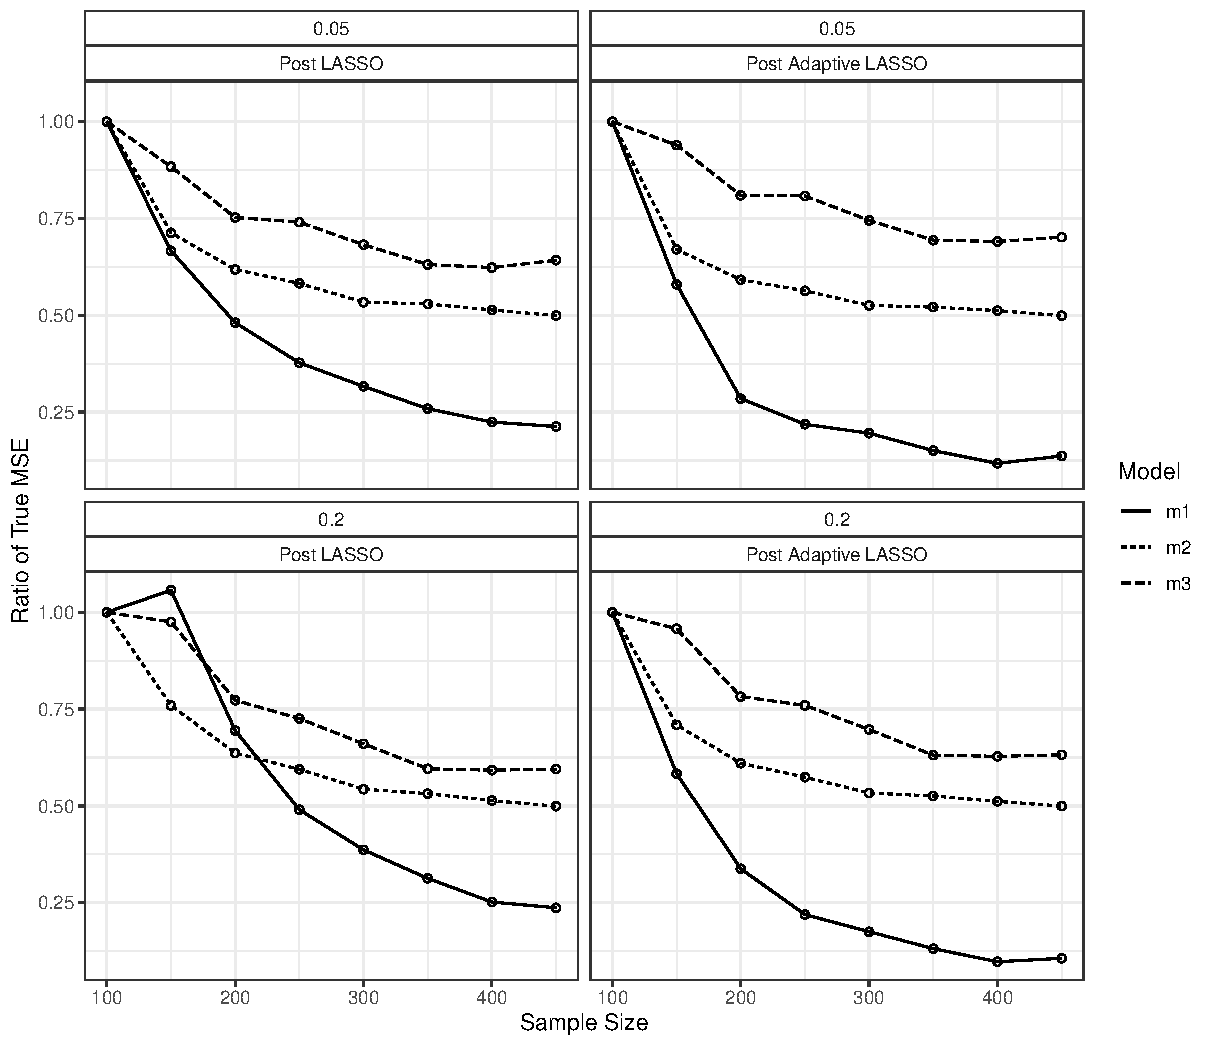
\includegraphics[width = 1\textwidth] {Graphics/rate.mean.plot.pdf}
		          %}
		          \caption{Comparison of convergence rates (using average MSEs)}
		          \label{rate.mean.plot}
	        \end{figure}

                In all panels of Figure \ref{rate.mean.plot}, it is observed that the ratios start at 1 and go downward with the increase of sample size, except for the case of $m_1$ and sample size 150 in the panel of $\sigma_2=20\%$ and post Lasso. This exception is assumed to originate from the influence of some extreme values. Such an influence is reduced in Figure \ref{rate.median.plot} when we use median MSEs instead. The downward ratios indicate that true MSE decreases with sample size, which is undoubtedly expected.\\

                Furthermore, it is obvious that in all panels, the ratios decrease the fastest for $m_1$, slower for $m_2$ and the slowest for $m_3$. This finding strongly corroborates Theorem \ref{convergence_rates_theorem} that our dimension adaptive estimator can always have the optimal convergence rate across different underlying models. In parametric underlying model ($m_1$), it has an optimal convergence rate of $n^{-1}$; in additive model ($m_2$), $n^{-\frac{2s}{2s+1}}$; and in unrestricted model ($m_3$), $n^{-\frac{2s}{2s+d}}$. All rates are up to an logarithmic factor. Actually, not only can we compare convergence rates across different underlying models, we are also able to verify the convergence rate for each model with the use of some data points in Figure \ref{rate.mean.plot}.\\

                Firstly, it is already known that in parametric underlying model ($m_1$), if the sample size grows from $n$ to $2n$, true MSE will be halved\footnote{We don't need to consider the constant in the rate, because it is generally the same for different sample size.}. That is, $\mathrm{MSE}(2n)/\mathrm{MSE}(n)=(2n)^{-1}/n^{-1}=1/2$. In the top-left panel of Figure \ref{rate.mean.plot}, it is clearly seen that when sample size increases from 100 to 200, the ratio decreases from 1 to 0.5; and when the sample size further increases to 400, the ratio is further halved, to around 0.25. This finding still holds in other three panels even with a little bit deviation. Since the evidence of convergence rate in parametric model at the top-left panel is very strong, we will focus on that panel for verification of convergence rates in other two models.\\

                It is further observed that for additive model ($m_2$), the ratio at sample size of 200 is around 0.625. That means, $\mathrm{MSE}(200)/\mathrm{MSE}(100)=(200)^{-\frac{2s}{2s+1}}/(100)^{-\frac{2s}{2s+1}}=2^{-\frac{2s}{2s+1}} \approx 0.625$. Then, we have $s \approx 1.05314$. With this approximation of $s$, we can verify any other point for $m_2$. For example, the observed ratio for sample size of 150 is around 0.75 on the plot. With the $s \approx 1.05314$, we have approximated ratio $\mathrm{MSE}(150)/\mathrm{MSE}(100)=1.5^{-\frac{2s}{2s+1}} \approx 1.5^{-0.67807} \approx 0.75962$. The approximated ratio coincides with the observed one, thus supporting the convergence rate in additive model, as found in our theorem.\\

                Finally, for unrestricted model ($m_3$), the ratio at sample size of 200 is observed to be about 0.75. It means, $\mathrm{MSE}(200)/\mathrm{MSE}(100)=(200)^{-\frac{2s}{2s+5}}/(100)^{-\frac{2s}{2s+5}}=2^{-\frac{2s}{2s+5}} \approx 0.75$. Then, we have $s \approx 1.77377$. Likewise, with this approximation of $s$, we can verify any other point for $m_3$. For instance, the observed ratio for sample size of 150 is about 0.875 on the plot, and with $s \approx 1.77377$, we have approximated ratio $\mathrm{MSE}(150)/\mathrm{MSE}(100)=1.5^{-\frac{2s}{2s+5}} \approx 1.5^{-0.41504} \approx 0.84512$. Again, observed and approximated ratios coincide roughly. This substantiates our theoretical finding of convergence rate in unrestricted model.

        \newpage
        
        \section{Application}\label{application}
            To make our dimension adaptive estimator much easier for empirical researchers to implement, we developed an R package \href{https://github.com/ccfang2/dimada}{dimada} which can be conveniently installed locally. Not only does it contain functions to generate sieves from original dataset and implement our estimator, but also it has functions to plot out and summarize the estimation results. In this section, with the R package, we perform our estimator on a real-life dataset and compare the out-of-sample empirical MSE with that of an OLS linear estimator ($ols$) and an additive estimator ($addt$).

            \subsection{Data}\label{data}
            The dataset consists of selling price and multiple attributes of cars. Our aim is to make prediction of car price based on the available attributes\footnote{We excluded four binary variables $diesel$, $electricity$, $hybrid$ and $petrol$ from original dataset. These variables include the information whether a car uses fuel or the specific resource. They are excluded because B-Spline sieves of these variables lead to some extreme values in estimated coefficients, which then influence out-of-sample MSEs. For sieves of other basis functions, there is no such influence. We computed out-of-sample MSEs with power series sieves and Legendre sieves of all variables from original dataset, and the results are consistent with those in Table \ref{out-of-sample_MSE}.}. The dataset is sourced from a data science online comminity, \href{https://www.kaggle.com/datasets/madhavmalhotra/car-price-regression-preprocessed}{Kaggle}. Table \ref{descriptive_stats} presents the descriptive statistics of our dataset.

            \begin{table}[!htbp] \centering 
                \caption{Descriptive statistics} 
                \label{descriptive_stats} 
                \scalebox{0.88}{
                \begin{threeparttable}
                \begin{tabular}{@{\extracolsep{5pt}}lcccccccc} 
                    \\[-1.8ex]
                    \hline 
                    \hline 
                    %\\[-1.8ex] 
                    & \multicolumn{1}{c}{Description} & \multicolumn{1}{c}{Type} & \multicolumn{1}{c}{Mean} & \multicolumn{1}{c}{St. Dev.} & \multicolumn{1}{c}{Min} & \multicolumn{1}{c}{Median} & \multicolumn{1}{c}{Max} \\ 
                    \hline  
                    $price$ & selling price (in \pounds) & cont.$^{a}$ & 23,469.940 & 16,406.720 & 450 & 18,999 & 145,000 \\ 
                    $year$ & production year & cont. & 2,016.738 & 2.884 & 1,997 & 2,017 & 2,020 \\ 
                    $mileage$ & mileage & cont. & 24,956.290 & 24,443.330 & 1 & 19,000 & 259,000 \\ 
                    $tax$ & sale tax (in \pounds) & cont. & 152.333 & 82.404 & 0 & 145 & 580 \\ 
                    $mpg$ & miles per gallon & cont. & 50.371 & 35.747 & 2.800 & 47.100 & 470.800 \\ 
                    $engine$ & size of engine (in litres) & cont. & 2.124 & 0.789 & 0.000 & 2.000 & 6.600 \\ 
                    \hline 
                    \hline
                \end{tabular} 
                \begin{tablenotes}
                    \footnotesize   %% If you want them smaller like foot notes
                    \item[a] "cont." stands for "continuous".
                \end{tablenotes}
                \end{threeparttable}
                }
            \end{table} 

            The total number of observations in this dataset is 4960, and there is no missing data. To compute out-of-sample empirical MSE, we split the original dataset into a train set ($60\%$, $2976$ observations) and a test set ($40\%$, $1984$ observations). As shown in Table \ref{descriptive_stats}, $price$ is the dependent variable and all other variables are regressors. 

            \subsection{Procedures}
            To apply our dimension adaptive estimator, it is worthy of mentioning that rescaling original regressors is required before sieve generation. The rule of variable selection in Lasso-type methods pertains to the magnitude of variables. In order to remove such an unfair influence, regressors have to be rescaled before analysis of Lasso\footnote{In our package \href{https://github.com/ccfang2/dimada}{dimada}, we use \href{https://glmnet.stanford.edu/}{glmnet} package to implement Lasso-type methods, which can actually be configurated to standardize regressors inside the command itself, so users usually do not need to standardize regressors beforehand. However, in our case, we have a separate test dataset which does not go through package \href{https://glmnet.stanford.edu/}{glmnet}, so it would be safer to rescale all regressors beforehand. It is unnecessary to standardize the dependent variable. But, the scale of dependent variable in this example is too large, we rescale it to have a small scale of errors for comparison.}. See Appendix \ref{standardization_of_lasso} for detailed discussions. Obviously, original regressors are not on the same scale, as seen in Table \ref{descriptive_stats}. In this section, we use z-score standardization to rescale original variables.\\
        
            With rescaled variables, we first generate sieves of regressors from a specific type of basis functions. Four types of basis functions are taken into account: power series, Legendre polynomials, B-splines and trigonometric polynomials. We consider interactions among all regressors when constructing sieves, so the maximum number of interacting regressors in a single term of sieves is 5. Usually, the number of basis functions generated for each single regressor is calculated directly from formula (\ref{set_of_basis_function}), where the lower bound of smoothness for different basis functions can be obtained from Corollary \ref{smoothness_corollary}. It then means 5 basis functions for each regressor when using power series or Legendre polynomials and 10 when using B-splines or trigonometric polynomials in this specific example. Nonetheless, in order to achieve better series approximation, we arbitrarily increase the number of basis functions for each regressor to 20\footnote{The number of basis functions for each regressor when using B-splines still remains to be 10, because in finite samples, higher number of B-splines doesn't necessarily mean better series approximation. If the number is too large, there will be some B-splines with only a few observations, leading to high approximation bias.}, instead of using the relatively low values computed directly from formula \ref{set_of_basis_function}. \\
        
            Then, Lasso-type methods are performed on the generated sieves, and significant terms are selected. Finally, to follow a common practice, post-selection OLS linear models are estimated on those selected terms, from which estimated coefficients can is used to compute out-of-sample MSEs on the separate test dataset.

            \subsection{Results}
            Figure \ref{dimada.trig.plot} portrays how cross-validated MSE changes with different number of non-zero coefficients for Lasso and adaptive Lasso within the train dataset. This is an example from using basis of trigonometric polynomials. The U-shape of curves signifies a trade-off between bias and variance of series approximation, and the shape of curves from using other basis functions is similar. As mentioned at the end of Section \ref{lasso}, cross validation is commonly used to choose the "best" regularization parameter $\lambda$, because it is pre-defined and researchers usually don't know how large it should be. As is indicated in Figure \ref{dimada.trig.plot}, the point with smallest cross-validated MSE is chosen, and the corresponding $\lambda$ and terms are selected. The number of selected terms is relatively large for basis trigonometric polynomials, which are bounded basis functions. \\

            Actually, the cross-validated empirical MSEs in Figure  \ref{dimada.trig.plot} are also out-of-sample MSEs which can be used for model evaluation, but the number of folds in cross-validation is 10, so the out-of-bag sample is of relatively small size ($=2976\times 0.1 \approx 298$). Therefore, a separate test dataset of larger size (=1984) is employed to examine the out-of-sample performance of our dimension adaptive estimator. 

            \begin{figure}[H] \centering
		      %\makebox[\textwidth][c]{
		      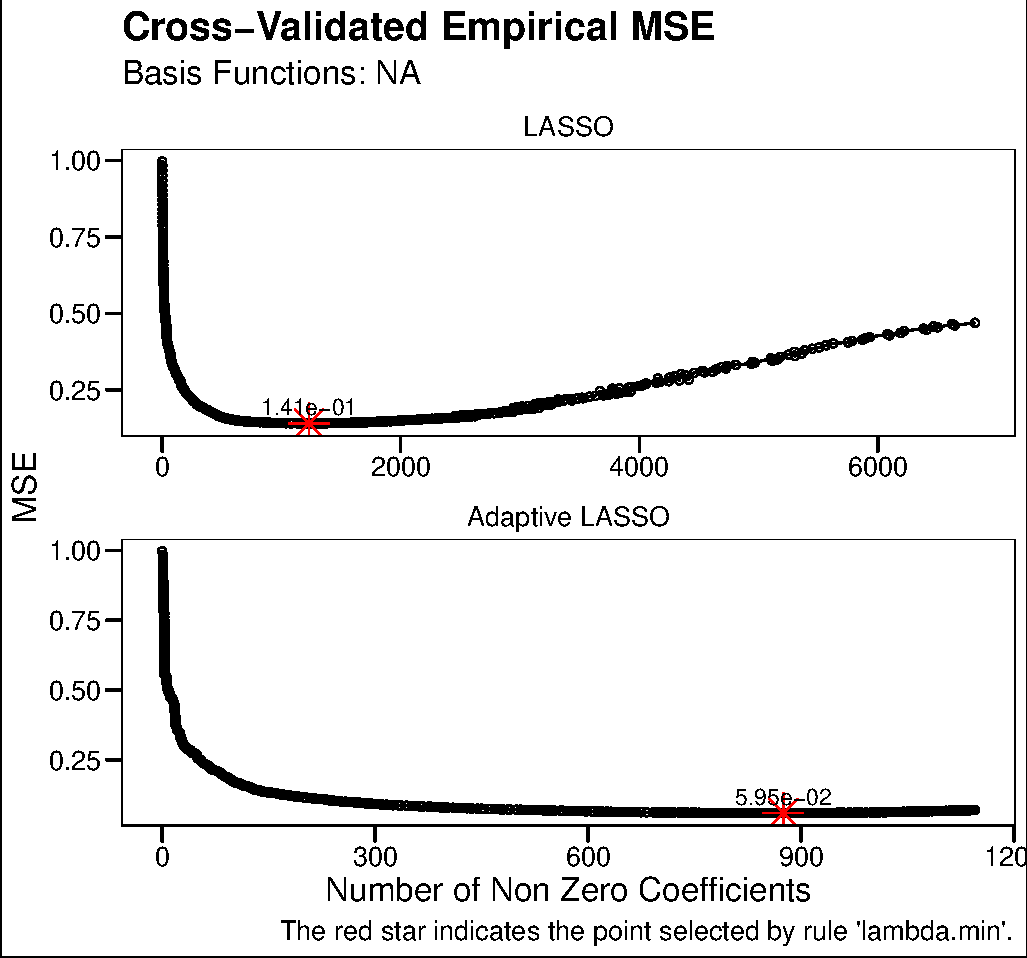
\includegraphics[width = 0.93\textwidth,trim= {{0.01\textwidth} {0.087\textwidth} {0.001\textwidth} {0.12\textwidth}}, clip=true]{Graphics/dimada.trig.plot.pdf}
		      %}
		      \caption{Cross-validated empirical MSE}
		      \label{dimada.trig.plot}
	    \end{figure}

            In Table \ref{out-of-sample_MSE}, the out-of-sample MSEs of our dimension adaptive estimator ($dimada$) on the separate test dataset are displayed, together with that of a simple OLS linear estimator ($ols$) and an additive estimator ($addt$). The definition and abbreviation of these estimators are consistent with those in Section \ref{simulation_study}. In the last column of Table \ref{out-of-sample_MSE}, we compute the ratio of each MSE to the MSE of OLS estimator.\\

            It is observed that the out-of-sample MSEs of estimator $addt$ are smaller than that of an OLS linear estimator, and the range of ratio is between $72.40\%$ to $85.57\%$, ignoring the outlier. This is because OLS estimator only considers linear relationship between regressors and the dependent variable while $addt$ estimator further considers non-linearity, even though both of them fail to include interactions among regressors.\\

            Moreover, the out-of-sample MSEs of our estimator $dimada$ are much smaller than that of $ols$, and the ratio ranges from $56.39\%$ to $72.75\%$. The performance of estimator $dimada$ varies greatly with the choice of basis functions. In this example, B-splines and trigonometric polynomials seem to perform better than power series and Legendre polynomials. For the same basis function, performance of $dimada$ is always better than $addt$. This indicates that the underlying model of this dataset is very likely not linearly parametric or additive, but non-parametric with interactions among regressors.

            \begin{table}[!htbp] \centering 
                \caption{Out-of-sample MSEs} 
                \label{out-of-sample_MSE} 
                \scalebox{0.88}{
                \begin{threeparttable}
                \begin{tabular}{lllcc}
                    \\[-1.8ex]
                    \hline
                    \hline
                    Estimator & Basis & Method & MSE & \multicolumn{1}{c}{MSE/MSE($ols$)} \\ 
                    \hline
                    $ols$ & & Linear OLS & $0.3181$ & $100\%$ \\
                    $addt$ & Power Series & Post LASSO  & $0.2719$ & $85.48\%$ \\
                    &  & Post Adaptive LASSO  & $0.2722$ & $85.57\%$ \\
                    & Legendre Polynomials & Post LASSO  & $0.2719$ & $85.47\%$ \\
                    &  & Post Adaptive LASSO  & $0.3232^a$ & $101.61\%^a$ \\
                    & B-Splines & Post LASSO  & $0.2303$ & $72.40\%$ \\
                    &  & Post Adaptive LASSO  & $0.2307$ & $72.52\%$ \\
                    & Trigonometric Polynomials & Post LASSO  & $0.2638$ & $82.92\%$ \\
                    &  & Post Adaptive LASSO  & $0.2636$ & $82.87\%$ \\
                    $dimada$ & Power Series & Post LASSO  & $0.2299$ & $72.27\%$ \\
                    &  & Post Adaptive LASSO  & $0.2296$ & $72.18\%$ \\
                    & Legendre Polynomials & Post LASSO  & $0.2314$ & $72.75\%$ \\
                    &  & Post Adaptive LASSO  & $0.2296$ & $72.18\%$ \\
                    & B-Splines & Post LASSO  & $0.1964$ & $61.74\%$ \\
                    &  & Post Adaptive LASSO  & $0.2011$ & $63.22\%$ \\
                    & Trigonometric Polynomials & Post LASSO  & $0.1897$ & $59.65\%$ \\
                    &  & Post Adaptive LASSO  & $0.1794$ & $56.39\%$ \\
                    \hline  
                    \hline
                \end{tabular}
                \begin{tablenotes}
                    \footnotesize   %% If you want them smaller like foot notes
                    \item[a] This MSE may be affected by some extreme values in the estimated coefficients of basis functions.
                \end{tablenotes}
                \end{threeparttable}
                }
            \end{table} 

            \subsection{Practical Suggestions}
            From the results of simulation and application, we summarize some suggestions for researchers who wish to apply our dimension adaptive estimator in their own studies.\\

            In the first step of generating a multivariate sieve space,
            \begin{enumerate}[label=\textbf{(\alph*)}, noitemsep]
                \item \textbf{Try different types of basis functions}. \\
                This can be configurated through the argument $basis$ in our R package \href{https://github.com/ccfang2/dimada}{dimada}, where there are 8 types of basis functions to choose from. There is no specific type that always works better than others, particularly in finite samples.  
                \item \textbf{Try different number of basis functions generated for each single regressor}.\\
                This corresponds to the argument $n.basis$ in our R package. By default, the formula (\ref{set_of_basis_function}) is used to compute the number of basis functions generated for each regressor. Usually, larger the number, better the series approximation. However, in finite samples, this may be violated, particularly for B-splines. If the number of knots for B-splines is too large, there might be some intervals with only a few observations, which result in poor approximation.
                \item \textbf{Consider interactions among regressors, unless it is certain that the model is additive}.\\
                This can be set with the argument $max.interaction$ in the R package. Economic variables are always entangled with other, so it is a good idea to consider interactions among them. When the number of regressors is not large, one can consider interactions among all variables. Nevertheless, if there are too many regressors, it is adviced to control the maximal number of interacting regressors in a single term under a certain value, such as 5 in order to expedite computation. 
                \item \textbf{Rescale all regressors with z-score standardization beforehand}.\\
                This is required if the original dataset is split into train and test datasets or there is a new dataset on which prediction needs to be made. Dependent variable doesn't need to be rescaled but if it is, remember to reverse it back to original scale after prediction.
            \end{enumerate}

            In the second step of applying Lasso-type methods,
            \begin{enumerate}[label=\textbf{(\alph*)}, noitemsep]
                \item \textbf{Use cross validation to select the "best" regularization parameter $\lambda$}\\
                In Lasso-type methods, instead of defining the regularization parameter $\lambda$ discretionarily, cross validation is usually used to choose the "best" $\lambda$ that gives the smallest out-of-bag MSE. This is also by default in our R package.
                \item \textbf{Use post-selection methods to obtain estimated coefficients for prediction, if necessary}.\\
                Since Lasso and adaptive Lasso are found to correctly recover the "right" sparsity of underlying model, we can estimate the model well in $\ell_2$-norm simply by doing an OLS (for linear model) restricted to the selected subset. It is a common practice to run the post-selection methods on chosen terms from Lasso-type methods. However, one needs to be cautious about doing inference with post-selection methods because they usually fail to provide uniform inference. \cite{Belloni_Chernozhukov_Hansen_2013} develop a "post-double-selection" method which has a property of uniform inference, but it is out of the scope of this thesis.
            \end{enumerate}
            
        \newpage
        \section{Conclusion}\label{conclusion}
            This thesis proposes a dimension adaptive estimator which can achieve an optimal convergence rate across all types of underlying models, inclusive of parametric, additive and unrestricted non-parametric models. Specifically, in parametric underlying model, it converges as fast as a parametric estimator, usually at a rate of $n^{-1}$, up to logarithmic factor. In additive and unrestricted non-parametric models, its convergence rate is slower but it still converges while parametric estimators do not converge to the true function. Hence, this estimator can perform as well as an "oracle" estimator in all underlying true models.\\

            This estimator is constructed with a two-step approach, as describe in Section \ref{estimation_steps}. To put it simply, the first step is to generate a multivariate sieve space from original regressors; the second step is to select significant terms in the sieve by Lasso-type methods. By applying a theorem in \cite{Bunea_2007},
            the oracle properties of the dimension adaptive estimator is established in Theorem \ref{convergence_rates_theorem}. Also, the required lower bound of smoothness for the unknown conditional mean function is different across various basis functions. This is summarised in Corollary \ref{smoothness_corollary}. \\

            The oracle properties of dimension adaptive estimator is strongly supported in the results of simulation. Furthermore, this estimator is applied in a real-life dataset about the prediction of car price. It is found that its performance is much better than an OLS linear estimator or an additive estimator in terms of out-of-sample MSE. Finally, practical suggestions are listed for researchers who are interested in using this estimator.\\

            This thesis has several limitations which may be considered in future research. First, the convergence rate usually has two portions multiplying together. The central portion is something related to the sample size $n$, such as $n^{-1}$. The other portion is a constant which is relative to smoothness $s$ and dimension $d$ of original data $X$, but not associated with $n$. However, in high dimensional analysis, $d$ sometimes grows with $n$, thus relating the "constant" portion to $n$. This may change the convergence rates discovered in Theorem \ref{convergence_rates_theorem}. It can be an interesting extension of the thesis. Second, cross validation is suggested in this thesis to select the "best" $\lambda$ for Lasso-type methods. However, the process of cross validation involves randomness in splitting data, which may be unwanted. Also, if the sample size is large, it may then be time-consuming to run cross validation. So, an alternative is to try Bayesian Information Criterion (BIC) instead. The performance of BIC in this research awaits to be tested. Last but not least, other types of basis functions needs to be discussed. In particularly, it is unknown how the lower bound of smoothness is defined for other basis functions except those in Corollary \ref{smoothness_corollary}.


        
        \newpage
	\section{Bibliography}
	    \printbibliography[heading=none]
        
        \newpage
        \section{Appendix}\label{appendix}
    \subsection{Standardization of Lasso}\label{standardization_of_lasso}
         In this section, we attempt to show that a standardization of regressors is required for an effective variable selection in Lasso. We use the same setting as shown in Section \ref{lasso}. $(Z_1, Y_1), \ldots, (Z_n,Y_n)$ is iid data with $Z_i \in \mathbb{R}^p$ and $Y_i \in \mathbb{R}$, following a linear model.
        \begin{align*}\label{linear_model}
            Y=\sum\limits_{j=1}^p Z_j\beta_j+\epsilon
        \end{align*}

        where $\beta_j$ are unknown coefficients. $Y=(Y_1, Y_2, \ldots, Y_n)^T$, $Z_j=(Z_{1j}, Z_{2j}, \ldots, Z_{nj})^{T}$ and $E[\epsilon|Z_1, Z_2, \ldots, Z_n]=0$. To save notation in the proof, we further assume that $Z_i$ does not contain a constant. Also, we have an orthonormality design, i.e., regressors are mutually orthonormal. To put it formally,
        \begin{align*}
            \frac{1}{n}Z^TZ=
            \begin{pmatrix}
                1 & 0 & \ldots & 0 \\
                0 & 1 & \ldots & 0 \\
                \vdots & \vdots & \ddots & \vdots \\
                0 & 0 & \ldots & 1 \\
            \end{pmatrix}
        \end{align*}
        where $Z=(Z_1,Z_2, \ldots, Z_j)$. Variances of all regressors $Z_j$ are normalized to 1. In this orthonormal design, it can be easily shown\footnote{Please refer to Section 2.4.1, \cite{Hastie_Tibshirani_Wainwright_2015} for details.} that a lasso estimate $\hat{\beta}_{\lambda, j}$ is
        \begin{align*}
            \hat{\beta}_{\lambda, j}=
            \begin{cases}
                \hat{\beta}_{OLS, j} + \lambda & \text{, if $\hat{\beta}_{OLS, j} < -\lambda$}\\
                0 & \text{, if $|\hat{\beta}_{OLS, j}| \le \lambda$}\\
                \hat{\beta}_{OLS, j} - \lambda & \text{, if $\hat{\beta}_{OLS, j} > \lambda$}\\
            \end{cases}
        \end{align*}
        where $\hat{\beta}_{OLS, j}=\frac{1}{n}\sum_{i=1}^n Z_{ij}Y_i$ is the coefficients estimated by OLS in this orthonormal design. It is seen that Lasso only selects regressor $Z_j$ if $|\hat{\beta}_{OLS, j}|=|\frac{1}{n}\sum_{i=1}^n Z_{ij}Y_i|>\lambda$. It means that the selection rule depends on the scale of coefficients. For example, if $Z_{1}$ is centered at 10000, while $Z_{2}$ is centered at 0, Lasso would unfairly prefer to selecting $Z_{1}$ since $|\frac{1}{n}\sum_{i=1}^n Z_{i1}Y_i|>\lambda$ even for a large $\lambda$. To remove such an unfair influence, it is required to standardize regressors beforehand.
        \begin{align*}
            \tilde{Z}_{ij}=\frac{Z_{ij}-\bar{Z}_j}{\hat{\sigma}_j}
        \end{align*}
        where $\hat{\sigma}_j$ is the standard deviation of $Z_j$. By using standardized $\tilde{Z}_{ij}$, the selection rule is not affected by the magnitude of variables, thus achieving an effective variable selection.
        


    \subsection{Derivation of $\kappa_M$ in Assumption \ref{dae_assumption_3}}\label{derivation_kappa}
        Let $g_k(X)=\prod_{l=1}^d p_{k_l}(x_l)$ denote basis functions with $1 \le k \le M$, and $g^M(X)=(g_1(X), \ldots, g_M(X))^T$ is the vector of all basis functions. Then, $\Psi_M=E[g^M(X)g^M(X)^{T}]$ in our setting. Let $v \in \mathbb{R}^M$, then
        \begin{align*}
            v^{T}\Psi_M v =& v^{T} E[g^M(X)g^M(X)^{T}]v\\
            =& E[(v^{T}g^M(X))^2]\\
            \ge & \frac{1}{C} \int_{\mathcal{X}}(v^{T}g^M(x))^2 dx\\
            = & \frac{1}{C} \int_{\mathcal{X}} \sum_{k=1}^{M}\sum_{j=1}^{M}v_kv_jg_k(x)g_j(x) dx\\
            = & \frac{1}{C}\sum_{k=1}^{M}v_k^2\\
            = & \frac{1}{C}v^{T}v
        \end{align*}

        To move from the second to the third line, we use the assumption that $||g_k(X)||=||\prod_{l=1}^d p_{k_l}(x_l)|| \ge c_0 = \frac{1}{C}$. To move from the fourth to fifth line, we use the orthonormality property of our basis functions. Moreover, 
        \begin{align*}
            v^{T}\mathrm{diag}(\Psi_M)v \le & C \int_{\mathcal{X}}\sum_{k=1}^M v_k^2 g_k(x)^2 dx\\
            =& C \sum_{k=1}^M v_k^2 \int_{\mathcal{X}} g_k(x)^2 dx\\
            =& Cv^{T}v
        \end{align*}

        In the first line, we use the assumption that $||g_k(X)||=||\prod_{l=1}^d p_{k_l}(x_l)|| \le C$. It follows that for any non-zero real vector $v$, we have
            \begin{align*}
                v^{T}\left(\Psi-\frac{1}{C^2}\mathrm{diag}(\Psi_M)\right)v=&v^{T}\Psi_Mv-\frac{1}{C^2}v^{T}\mathrm{diag}(\Psi_M)v\\
                \ge & \frac{1}{C}v^{T}v-\frac{1}{C}v^{T}v\\
                =&0
            \end{align*}
                        
        Therefore, there exists a constant $\kappa_M=\frac{1}{C^2}>0$ such that $\Psi_M-\kappa_M\mathrm{diag}(\Psi_M)$ is positive semi-definite. Assumption \ref{assumption_3} is thus guaranteed. It is noted that orthonormality of basis functions simplifies the expression of $\kappa_M$, but even if basis functions are not orthonormal, there can exist such a $\kappa_M>0$ that makes $\Psi_M-\kappa_M\mathrm{diag}(\Psi_M)$ positive semi-definite, though probably with a more complicated derivation process and expression.

    \subsection{Proof of Corollary \ref{smoothness_corollary}}\label{proof_of_corollary}
        \subsubsection{Normalized Legendre Polynomials}\label{normalized_legendre}

        \textbf{Step 1: Deriving $L$ and $L_0$ in Assumption \ref{dae_assumption_2}}\\
        By definition, Legendre polynomials are orthogonal with respect to a uniform density on $[-1,1]$ (\cite{Hansen_2022}). Suppose $p_k(X)$ ($k=0,1,2,\ldots$) are Legendre polynomials defined on interval $[-1,1]$. By fixing $p_k(1)=1$, we have\footnote{\url{https://en.wikipedia.org/wiki/Legendre_polynomials}}:
        \begin{align*}
            \int_{-1}^1 p_j(x)p_k(x)\diff x=\frac{2}{2k+1} \delta_{jk}
        \end{align*}
        where $\delta_{jk}$ denotes Kronecker delta\footnote{Kronecker delta is a function of two variables, which are usually non-negative integers. The function is 1 if the two variables equal, and is 0 otherwise. For example, $\delta_{12}=0$, because $1 \not= 2$; while $\delta_{11}=1$, because $1=1$.}, which equals to 1 if $j=k$, and equals to 0 otherwise. That means, the squared $L_2$ norm of $p_k(X)$ on $[-1,1]$ is:
        \begin{align*}
            ||p_k(X)||^2=\int_{-1}^1 p_k(x)^2 \diff x = \frac{2}{2k+1}
        \end{align*}
        where $||\cdot||$ denotes $L_2$ norm. Then, if we further normalize the Legendre polynomials $p_k(X)$, we have $\tilde{p}_k(X)=\sqrt{\frac{2k+1}{2}}p_k(X)$ such that:
        \begin{align*}
            ||\tilde{p}_k(X)||^2=\int_{-1}^1 \tilde{p}_k(X)^2 \diff x =\int_{-1}^1 \left(\sqrt{\frac{2k+1}{2}}p_k(x)\right)^2 \diff x =\frac{2k+1}{2}||p_k(X)||^2=1
        \end{align*}
        Therefore, $\tilde{p}_k(X)$ ($k=0,1,2,\ldots$) are normalized Legendre polynomials that are discussed in Corollary \ref{smoothness_corollary}. They are orthonormal. In Figure \ref{legendre_poly_plot}, it is seen that Legendre polynomials $p_k(X)$ are bounded above by 1, so for normalized Legendre polynomials, we have:
        \begin{align*}
            ||\tilde{p}_k(X)||_{\infty}=\left|\left|\sqrt{\frac{2k+1}{2}}p_k(X)\right|\right|_{\infty} \le \sqrt{\frac{2k+1}{2}}
        \end{align*}
         In other words, $||\tilde{p}_k||_{\infty} \lesssim \sqrt{k}$. As a consequence, the $L_{\infty}$ norm of basis functions in our multivariate sieve space is $||\prod_{l=1}^d \tilde{p}_{k_l}||_{\infty} \lesssim \sqrt{\prod_{l=1}^dk_l}$. Because $\sum_{l=1}^dk_l \lesssim n^{\frac{1}{2\underline{s}+1}}$ with reference to (\ref{set_of_basis_function}), we can maximize the product $\prod_{l=1}^dk_l$ by having $k_l=\frac{1}{d}n^{\frac{1}{2\underline{s}+1}}$. Then,
         \begin{align*}
             \left|\left|\prod_{l=1}^d \tilde{p}_{k_l}\right|\right|_{\infty} \lesssim n^{\frac{d}{4\underline{s}+2}}
         \end{align*}
         As a result, according to Assumption \ref{dae_assumption_2}, we have $L=n^{\frac{d}{4\underline{s}+2}}$ and $L_0=L^2=n^{\frac{d}{2\underline{s}+1}}$.\\

        \textbf{Step 2: Discussing the first part of inequality about $\pi_{n,M}(\beta)$ in (\ref{pi_n_M})}
        
        To make $\pi_{n,M}(\beta)$ asymptotically zero, it is sufficient to make its upper bound to be asymptotically zero. There are two parts in its upper bound, then it is sufficient to have both parts going to zero in the limit. Ignoring constants, the first part of upper bound of $\pi_{n,M}(\beta)$ is
        \begin{align*}
            &M^2\exp\left( -\min\left\{ nr_{n,M}^2, \frac{nr_{n,M}}{L}, \frac{n}{L^2}, \frac{n}{L_0M^2(\beta)},\frac{n}{L^2M(\beta)} \right\} \right)\\
            =& M^2 \exp\left( -\min\left\{ A^2\log M, A \sqrt{\log M} n^{\frac{1}{2}-\frac{d}{4\underline{s}+2}}, n^{1-\frac{d}{2\underline{s}+1}},n^{1-\frac{d}{2\underline{s}+1}}M^{-2}(\beta), n^{1-\frac{d}{2\underline{s}+1}}M^{-1}(\beta)\right\} \right)\\
            =& M^2 \exp\left( -\min\left\{ A^2\log M, A \sqrt{\log M} n^{\frac{1}{2}-\frac{d}{4\underline{s}+2}}, n^{1-\frac{d}{2\underline{s}+1}},n^{1-\frac{d}{2\underline{s}+1}-\frac{2d}{2s+d}}, n^{1-\frac{d}{2\underline{s}+1}-\frac{d}{2s+d}}\right\} \right)
        \end{align*}
        To move from the first to second line, we use $L=n^{\frac{d}{4\underline{s}+2}}$ and $L_0=n^{\frac{d}{2\underline{s}+1}}$ for normalized Legendre polynomials. To move from the second to third line, we use $M(\beta)=n^{\frac{d}{2s+d}}$ because it is the largest among all three types of underlying models. A sufficient condition for this upper bound to be asymptotically zero is that all terms within the brace should go to infinity, otherwise the upper bound is not asymptotically zero. The terms $A^2\log M$ is naturally non-zero. Then the sufficient condition is reduced to
        \[
        \left\{
            \begin{array}{cc}
                \frac{1}{2}-\frac{d}{4\underline{s}+2} & \ge0 \\
                1-\frac{d}{2\underline{s}+1} & >0 \\
                1-\frac{d}{2\underline{s}+1}-\frac{2d}{2s+d} & > 0\\
                1-\frac{d}{2\underline{s}+1}-\frac{d}{2s+d}& > 0\\
                \underline{s}&\ge0\\
            \end{array}
        \right.
        \]
        If this set of inequalities works for $\underline{s}$, then it should work for all $s$. So, we can replace $s$ with $\underline{s}$. Then, by solving this set of inequalities, we have
        \begin{align*}
            \underline{s} > \frac{2d-1+\sqrt{8d^2+1}}{4}
        \end{align*}
        For example, when $d=2$, we need $\underline{s}>2.187$ to maintain the optimal convergence rate in Theorem \ref{convergence_rates_theorem}. The formula is a little bit complicated, but we can find a simpler sufficient condition.
        \begin{align*}
            \underline{s}\ge\frac{3d-1}{2}
        \end{align*}
        This is a sufficient condition because $\frac{3d-1}{3}>\frac{2d-1+\sqrt{8d^2+1}}{4}$ for all $d \in \{1,2,\ldots\}$. It is worthy of mentioning that the above condition is derived from using $M(\beta)=n^{\frac{d}{2s+d}}$, which is the largest $M(\beta)$ in all three underlying models. \\
                        
        Hence, even if $\underline{s} \le \frac{2d-1+\sqrt{8d^2+1}}{4}$, it can still help to maintain the optimal convergence rate in additive and parametric model. By following a similar argument as above but with $M(\beta)=n^{\frac{1}{2\underline{s}+1}}$, we have a sufficient condition $\underline{s}\ge \frac{d+1}{2}$, which is smaller than the lower bound for maintaining convergence rate in all three models. Likewise, if we only need the optimal convergence rate to hold in parametric model, then we can use $M(\beta)=K^d$ with $K$ being a positive constant. The resulting condition is $\underline{s}> \frac{d-1}{2}$. \\

        \textbf{Step 3: Discussing the second part of inequality about $\pi_{n,M}(\beta)$ in (\ref{pi_n_M})}

        Regarding the second part of upper bound of $\pi_{n,M}(\beta)$, we have
        \begin{align*}
            \exp\left( -\frac{M(\beta)}{L^2(\beta)}nr_{n,M}^2 \right)=\exp\left( -\frac{M(\beta)}{L^2(\beta)}A^2\log M \right)
        \end{align*}
        where $L(\beta)=||f-f_{\beta}||_{\infty}$. With reference to the formula (3.7) in \cite{Belloni_Chernozhukov_Chetverikov_Kato_2015}, we have $L(\beta) \lesssim M(\beta)^{-\frac{s}{d}}$. Then, 
        \begin{align*}
            \frac{M(\beta)}{L^2(\beta)} \gtrsim M(\beta)^{\frac{2s+d}{d}} = n^{\frac{d}{2s+d}\frac{2s+d}{d}}=n
        \end{align*}
        where we use $M(\beta)=n^{\frac{d}{2s+d}}$. Obviously, the second part is asymptotically zero, too. The result also holds when $M(\beta)=n^{\frac{1}{2s+1}}$ or $K^d$. The intuitive explanation is that when $n \rightarrow \infty$, the $L_{\infty}$ norm of approximation error $L(\beta)$ goes to zero, and the number of coefficients $M(\beta)$ goes to infinity, thus making $\frac{M(\beta)}{L^2(\beta)}$ goes to infinity. 
        
        \subsubsection{Orthonormalized B-Splines}\label{orthonormalized_b-splines}

        \textbf{Step 1: Deriving $L$ and $L_0$ in Assumption \ref{dae_assumption_2}}\\
        In Appendix \ref{orthogonal_b_splines}, it is shown that on $[a,b]$, the squared $L_2$ norm of orthogonal B-Splines $||P_k||^2$ are bounded above. From the example in Table \ref{example_values_n_k}, it is further observed that $||P_k||^2$ grows with $k$. Hence, if $P_k$ is normalized, the resulting orthonomalized B-Splines $\tilde{P}_k$ would have an $L_{\infty}$ norm that goes downward with $k$. Then, it is bounded above, supposedly by a constant $C$. As a consequence, the $L_{\infty}$ norm of basis functions in multivariate sieve space is $||\prod_{l=1}^d \tilde{P}_{k_l}||_{\infty} \lesssim C^d$. According to Assumption \ref{dae_assumption_2}, we have $L=C^d$ and $L_0=L^2=C^{2d}$. \\
    
        \textbf{Step 2: Discussing the first part of inequality about $\pi_{n,M}(\beta)$ in (\ref{pi_n_M})}\\
        Again, it is sufficient to argue that both parts of the upper bound of $\pi_{n,M}(\beta)$ goes to zero in the limit. Ignoring constants, the first part is
        \begin{align*}
            &M^2\exp\left( -\min\left\{ nr_{n,M}^2, \frac{nr_{n,M}}{L}, \frac{n}{L^2}, \frac{n}{L_0M^2(\beta)},\frac{n}{L^2M(\beta)} \right\} \right)\\
            =& M^2\exp\left( -\min\left\{ A^2 \log M, A\sqrt{\log M}C^{-d}n, C^{-2d}n, C^{-2d}nM^{-2}(\beta), C^{-2d}nM^{-1}(\beta) \right\} \right)\\
            =& M^2\exp\left( -\min\left\{ A^2 \log M, A\sqrt{\log M}C^{-d}n, C^{-2d}n, C^{-2d}n^{1-\frac{2d}{2s+d}}, C^{-2d}n^{1-\frac{d}{2s+d}} \right\} \right)
        \end{align*}

        To move from the first to second line, we use $L=C^d$ and $L_0=C^{2d}$ for orthonormalized B-splines. To move from the second to third line, we use $M(\beta)=n^{\frac{d}{2s+d}}$ because it is the largest among all three underlying models. Again, a sufficient condition is that all terms should go to infinity. The terms $A^2 \log M$, $A\sqrt{\log M}C^{-d}n$ and $C^{-2d}n$ are nonzero, so the condition is reduced to 
        \[
            \left\{
            \begin{array}{cc}
                1-\frac{2d}{2s+d} &> 0\\
                1-\frac{d}{2s+d} &> 0\\
                \underline{s} &\ge 0
            \end{array}
            \right.
        \]
        We need to replace $s$ with the lower bound of smoothness, i.e., $\underline{s}$, so this set of inequalities should work for all $s$. By solving this set of inequalities, we have
        \begin{align*}
            \underline{s} >\frac{d}{2}
        \end{align*}
        A sufficient condition is $\underline{s}\ge \frac{d+1}{2}$. For example, when $d=2$, we need $\underline{s}\ge1.5$ to maintain the convergence rate in Theorem \ref{convergence_rates_theorem}; when $d=10$, we need $\underline{s}\ge5.5$. This restriction is less stricter than that for normalized Legendre polynomials. If we only need optimal convergence rate for additive and parametric model, we can use $M(\beta)=n^{\frac{1}{2s+1}}$ instead. The resulting condition is $\underline{s}>\frac{1}{2}$. By following a similar argument, we find out we don't need any further restriction on $\underline{s}$ except that $\underline{s}\ge0$ if we only need an optimal rate in parametric model. \\

        \textbf{Step 3: Discussing the second part of inequality about $\pi_{n,M}(\beta)$ in (\ref{pi_n_M})}

        Regarding the second part of upper bound of $\pi_{n,M}(\beta)$, we can verify that it goes to zero with $n \rightarrow \infty$ in the same way as we argue in Section \ref{normalized_legendre}. 

        \subsubsection{Normalized Haar wavelets}\label{normalized_haar_wavelets}
        As shown in Section \ref{haar_wavelets}, normalized Haar basis functions are denoted as $\psi_{jk}(X)$. They are orthogonal with respect to $[0,1]$, by design. With normalization, the $L_{\infty}$ norm of Haar basis functions becomes $||\psi_{jk}(X)||_{\infty}=2^{j/2}$. Let $k^{\prime}$ be the total number of basis functions in all levels of Haar wavelets up to the level of $j$, then $k^{\prime}=2^{j+1}$, which means $j=\log_2k^{\prime}-1$. The $L_{\infty}$ norm becomes:
        \begin{align*}
            ||\psi_{jk}(X)||_{\infty}=2^{\frac{\log_2k^{\prime}-1}{2}}=2^{-1/2}2^{\log_2\sqrt{k^{\prime}}}=2^{-1/2}\sqrt{k^{\prime}} \lesssim \sqrt{k^{\prime}}
        \end{align*}
        It is found that the derived condition of $L_{\infty}$ norm for normalized Haar wavelets coincides with that for normalized Legendre polynomials. As a consequence, the same $L$ and $L_0$ are obtained, i.e., $L=n^{\frac{d}{4\underline{s}+2}}$ and $L_0=L^2=n^{\frac{d}{2\underline{s}+1}}$. All other proof for normalized Legendre polynomials in Section \ref{normalized_legendre} also apply in this section.

        \subsubsection{Normalized Trigonometric Polynomials}\label{normalized_trig_poly}
        First, we can show that the system $\mathcal{T}:=\{1, \cos(\pi X), \sin(\pi X), \cos(2\pi X), \sin(2\pi X),\ldots\}$ is a complete orthogonal system for $X \in [-1,1]$. In order to prove the orthogonality of this system, we have to show\footnote{The basis 1 is naturally orthogonal to other bases on the domain $[-1,1]$.}
        \begin{align*}
        \begin{cases}
            \int_{-1}^1 \cos(m\pi x)\cos(n\pi x)\diff x=0, & m,n \in \mathbb{Z}_{+}, m \not=n\\
            \int_{-1}^1 \sin(m\pi x)\sin(n\pi x)\diff x=0, & m,n \in \mathbb{Z}_{+}, m \not=n\\
            \int_{-1}^1 \cos(m\pi x)\sin(n\pi x)\diff x=0, & m,n \in \mathbb{Z}_{+}, m \not=n
        \end{cases}
        \end{align*}

        To show the second integral, we use the following product-to-sum trigonometric identity.
        \begin{align*}
            \sin A \sin B=\frac{\cos(A-B)-\cos(A+B)}{2}
        \end{align*}

        So, if $m,n\ge 1$ and $m \not=n$, we have
        \begin{align*}
            \int_{-1}^1 \sin(m\pi x)\sin(n\pi x)\diff x =& \int_{-1}^1 \frac{\cos\left((m-n)\pi x\right)-\cos\left((m+n)\pi x\right)}{2}\diff x\\
            =& \frac{1}{2}\left[\frac{\sin\left((m-n)\pi x\right)}{m-n}-\frac{\sin\left((m+n)\pi x\right)}{m+n}\right]_{-1}^1\\
            =&0
        \end{align*}

        Likewise, the other two integrals can be solved by using the following identities.
        \begin{align*}
        \begin{cases}
            \cos A \cos B=&\frac{\cos(A-B)+\cos(A+B)}{2}\\
            \cos A \sin B=&\frac{\sin(A+B)-\sin(A-B)}{2}
        \end{cases}
        \end{align*}

        Also, for $m,n\ge1$ and $x \in [-1,1]$, we have $||1||^2=2$, $||\cos(m\pi x)||^2=\pi$ and $||\sin(n\pi x)||^2=\pi$. Therefore, to normalize the system $\mathcal{T}$ of trigonometric polymials, we would have a new system $\tilde{\mathcal{T}}=\{1/\sqrt{2}, \cos(\pi X)/\sqrt{\pi}, \sin(\pi X)/\sqrt{\pi}, \cos(2\pi X)/\sqrt{\pi}, \sin(2\pi X)/\sqrt{\pi},\ldots\}$. This is then an orthonormal system. Moreover, as $\cos(m\pi x)$ and $\cos(n\pi x)$ is bounded above by 1, the $L_{\infty}$ norm of basis functions in the new system $\tilde{\mathcal{T}}$ is then bounded above by $1/\sqrt{2}$, which is a constant. Consequently, $L$ and $L_0$ in Assumption \ref{dae_assumption_2} are also constant, thus making the rest of proof the same as that in Section \ref{orthonormalized_b-splines} for orthonormalized B-splines.\\

        To conclude, all basis functions we use in this section are orthonormalized only for the consolidation and simplicity of proof. If basis functions are not orthonormal, Theorem \ref{convergence_rates_theorem} can still hold but with some changes to parameters. For example, if we don't normalize Legendre polynomials, $L$ and $L_0$ are then constants, and $\kappa_M$ is not $1/C^2$ any more. This may change the lower bound of smoothness in Corollary \ref{smoothness_corollary}. In practical implementation of our dimension adaptive estimation, it is not a must to orthonormalize basis functions.

    \newpage
    \subsection{Orthogonal B-splines}\label{orthogonal_b_splines}
        In this section, we are going to show that the squared $L_2$ norm of orthogonal B-splines are bounded below and above. To simplify our proof, we use linear B-splines, but the result also applies to B-splines with higher orders with more notation. The main idea of this proof is from \cite{Mason_1993}.\\

        Suppose a family of linear B-splines $\{L_k\} (k=0,\ldots,n)$ is defined on $[a,b]$, and the set of ordered knots $\{x_k\}$ with $x_{-1}<x_0=a$ and $b=x_n<x_{n+1}$. Then, $L_k$ is continuous in $[x_{k-1},x_{k+1}]$, and by normalization we assume that $L_k(x_k)=1$. Now, we hope to convert the linear B-splines $\{L_k\}$ to a basis of orthogonal splines. Typically, it can be done by the following recurrence:
        \begin{align*}
            P_0=&L_0\\
            P_k=&L_k-a_{k-1}P_{k-1} \quad (k=1,\ldots,n)
        \end{align*}
        where $P_k$ is orthogonal linear B-splines with support $[a,x_{k+1}]$ and $a_{k-1}$ are undetermined parameters. Then, we need to determine the values of $a_{k-1}$. The inner product $\langle P_r,L_k\rangle=0$ $(r \le k-2)$ because $P_r$ and $L_k$ have disjoint supports. Hence, it is sufficient to have
        \begin{align*}
            \langle P_k,P_{k-1}\rangle=& \langle L_k-a_{k-1}P_{k-1}, P_{k-1}\rangle
            = \langle L_k,P_{k-1}\rangle-a_{k-1}||P_{k-1}||^2
        \end{align*}
        Then, we have $\langle L_k,P_{k-1}\rangle-a_{k-1}||P_{k-1}||^2$. Denote $n_k=||P_k||^2=\langle P_k,P_k\rangle$ and $v_k=\langle L_{k+1}, P_k\rangle$. So, $v_k=a_kn_k$. It is noted that $\langle L_{k+1}, P_k\rangle=\langle L_{k+1}, L_k-a_{k-1}P_{k-1}\rangle=\langle L_{k+1},L_k\rangle$ due to $\langle L_{k+1},P_{k-1}\rangle=0$, then $v_k=\langle L_k,L_{k+1}\rangle$ too. Thus, the squared $L_2$ norm of $P_k$ is 
        \begin{align*}
            n_k=&\langle P_k,P_k\rangle\\
            =&\langle L_k-a_{k-1}P_{k-1},L_k-a_{k-1}P_{k-1}\rangle\\
            =&\langle L_k,L_k\rangle-2a_{k-1}\langle L_k,P_{k-1}\rangle+a_{k-1}^2\langle P_{k-1},P_{k-1}\rangle\\
            =&u_k-2a_{k-1}v_{k-1}+a_{k-1}^2n_{k-1}\\
            =&u_k-2a_{k-1}v_{k-1}+a_{k-1}v_{k-1}\\
            =&v_k-a_{k-1}v_{k-1}
        \end{align*}

        where $v_k$ and $u_k$ are computable constants and should be bounded due to the property of B-splines. By using $v_k=a_kn_k$ and $n_k=u_k-a_{k-1}v_{k-1}$, we can solve for $n_k$ and $a_k$ $(k=0,1,\ldots,n-1)$:
        \begin{align*}
            n_0=&u_0\\
            a_k=&\frac{v_k}{n_k}\\
            n_{k+1}=&u_{k+1}-a_kv_k
        \end{align*}

        Note that $\{a_k\}$ can be alternatively eliminated. Then, we have
        \begin{align*}
            n_0=&u_0\\
            n_k=&u_k-\frac{v_{k-1}^2}{n_{k-1}} \quad (k=1,\ldots,n-1) 
        \end{align*}

        Obviously, $n_k$ is bounded above since $u_k$ is bounded above and $\frac{v_{k-1}^2}{n_{k-1}}\ge0$; $n_k$ is also bounded below since it is a squared $L_2$ norm. To put it formally, there exists constants $C_1$ and $C_2$ such that $C_1 \le n_k \le C_2$ for $k=0,1,\ldots,n-1$.\\

        \cite{Mason_1993} also presents an example by giving explicit values to constants $u_k$, $v_k$ and formulae for $\{L_k\}$. Denote $h_k=x_k-x_{k-1}$, and they show
        \[
            L_k(x)=
            \left\{
            \begin{array}{cc}
                (h_k)^{-1}(x-x_{k-1}), &x \in [x_{k-1},x_k]\\
                (h_{k+1})^{-1}(x_{k+1}-x), &x \in [x_k,x_{k+1}]
                \end{array}
            \right.
        \]
        and
            \begin{align*}
                u_0=&\frac{1}{3}h_1\\
                u_k=&\frac{1}{3}(h_k+h_{k+1}) \quad (k=1,\ldots,n-1)\\
                u_n=&\frac{1}{3}h_n\\
                v_k=&\frac{1}{6}h_{k+1} \quad (k=0,\ldots,n-1)
            \end{align*}
        Hence, it gives rise to the following equations: $n_0=\frac{1}{3}h_1$ and $n_k=\frac{1}{3}(h_k+h_{k+1})-\frac{h_{k}^2}{36n_{k-1}}$ for all $k=1,\ldots,n-1$. Without loss of generality, assume $h_k=1$ for all $k$, then the explicit values of $n_k$ are as follows.
                
	\begin{table}[H]
		\centering
            \caption{Example Values of $n_k$}
            \label{example_values_n_k}
		\begin{tabular}{lcccccccc}
                \hline
                \hline
			$k$	& 1 & 2 & 3 & 4 & 5 & 6 & 7 & 8 \\
                \hline
			$n_k$ & 0.33333 & 0.58333 & 0.61905 & 0.62180 & 0.62199 & 0.622010 & 0.622010 & 0.622010\\
			\hline
                \hline
		\end{tabular}
	\end{table}
        
        In Table \ref{example_values_n_k}, values of $n_k$ are observed to converge to 0.622010 in this specific example, testifying the existence of an upper bound.

    \newpage
    \subsection{Additional Tables}
    \begin{table}[!htbp] \centering 
        \caption{Median of out-of-sample empirical MSE for $m_1$} 
        \label{mse_median_m1} 
        \scalebox{0.815}{
        \begin{threeparttable}
        \begin{tabular}{llcccccccc}
            \\[-1.8ex]
            \hline
            \hline
            & & \multicolumn{4}{c}{$\sigma_1=5\%$} & \multicolumn{4}{c}{$\sigma_2=20\%$} \\ 
            & & \multicolumn{2}{c}{Post} & \multicolumn{2}{c}{Post Adaptive} & \multicolumn{2}{c}{Post} & \multicolumn{2}{c}{Post Adaptive} \\ 
            & & \multicolumn{2}{c}{LASSO} & \multicolumn{2}{c}{LASSO} & \multicolumn{2}{c}{LASSO} & \multicolumn{2}{c}{LASSO} \\ 
            Basis & Estimator & MSE & Terms$^b$ & MSE & Terms$^b$ & MSE & Terms$^b$ & MSE & \multicolumn{1}{c}{Terms$^b$} \\ 
            \hline
            Power Series & $dimada$  & $0.002622$ & $17$ & $0.002537$ & $5$ & $0.04180$ & $17$ & $0.04067$ & $5$ \\
            & $addt$  & $0.002561$ & $7$ & $0.002537$ & $5$ & $0.04091$ & $8$ & $0.04060$ & $5$ \\
            & $ols^a$ & \textbf{0.002537} & $5$ & \textbf{0.002537} & $5$ & \textbf{0.04060} & $5$ & \textbf{0.04060} & $5$ \\
            Legendre & $dimada$  & $0.002616$ & $17$ & $0.002537$ & $5$ & $0.04194$ & $16$ & $0.04068$ & $5$ \\
            & $addt$  & $0.002554$ & $7$ & $0.002537$ & $5$ & $0.04105$ & $8$ & $0.04060$ & $5$ \\
            & $ols^a$ & \textbf{0.002537} & $5$ & \textbf{0.002537} & $5$ & \textbf{0.04060} & $5$ & \textbf{0.04060} & $5$ \\
            B-Splines & $dimada$  & $0.010528$ & $191$ & $0.009168$ & $107$ & $0.10267$ & $130$ & $0.08736$ & $94$ \\
            & $addt$  & $0.002676$ & $28$ & $0.002678$ & $25$ & $0.04282$ & $28$ & $0.04308$ & $25$ \\
            & $ols^a$ & \textbf{0.002537} & $5$ & \textbf{0.002537} & $5$ & \textbf{0.04060} & $5$ & \textbf{0.04060} & $5$ \\
            Trigonometric & $dimada$  & $0.006139$ & $159$ & $0.004363$ & $14$ & $0.05596$ & $42$ & $0.05487$ & $33$ \\
            & $addt$ & $0.006612$ & $12$ & $0.006563$ & $10$ & $0.04397$ & $20$ & $0.04387$ & $11$ \\
            & $ols^a$ & \textbf{0.002537} & $5$ & \textbf{0.002537} & $5$ & \textbf{0.04060} & $5$ & \textbf{0.04060} & $5$ \\
            \hline 
            \hline
        \end{tabular}
        \begin{tablenotes}
            %\footnotesize   %% If you want them smaller like foot notes
            \item [a] The $ols$ estimator doesn't involve any basis function or Lasso-type methods.
            \item [b] Average number of selected terms with non-zero coefficients.
        \end{tablenotes}
        \end{threeparttable}
        }
    \end{table} 

    \begin{table}[!htbp] \centering 
        \caption{Median of out-of-sample empirical MSE for $m_2$} 
        \label{mse_median_m2} 
        \scalebox{0.85}{
        \begin{threeparttable}
        \begin{tabular}{llcccccccc}
            \\[-1.8ex]
            \hline
            \hline
            & & \multicolumn{4}{c}{$\sigma_1=5\%$} & \multicolumn{4}{c}{$\sigma_2=20\%$} \\ 
            & & \multicolumn{2}{c}{Post} & \multicolumn{2}{c}{Post Adaptive} & \multicolumn{2}{c}{Post} & \multicolumn{2}{c}{Post Adaptive} \\ 
            & & \multicolumn{2}{c}{LASSO} & \multicolumn{2}{c}{LASSO} & \multicolumn{2}{c}{LASSO} & \multicolumn{2}{c}{LASSO} \\ 
            Basis & Estimator & MSE & Terms$^b$ & MSE & Terms$^b$ & MSE & Terms$^b$ & MSE & \multicolumn{1}{c}{Terms$^b$} \\ 
            \hline
            Power Series & $dimada$  & $0.17097$ & $37$ & $0.16437$ & $18$ & $0.2133$ & $38$ & $0.2016$ & $19$ \\
            & $addt$ & \textbf{0.14298} & $13$ & \textbf{0.14767} & $9$ & \textbf{0.1820} & $13$ & \textbf{0.1844} & $9$ \\
            & $ols^a$ & $0.74993$ & $5$ & $0.74993$ & $5$ & $0.7876$ & $5$ & $0.7876$ & $5$ \\
            Legendre & $dimada$ & $0.17357$ & $41$ & $0.16556$ & $22$ & $0.2154$ & $41$ & $0.2066$ & $23$ \\
            & $addt$ & \textbf{0.14379} & $12$ & \textbf{0.14612} & $10$ & \textbf{0.1824} & $12$ & \textbf{0.1846} & $10$ \\
            & $ols^a$ & $0.74993$ & $5$ & $0.74993$ & $5$ & $0.7876$ & $5$ & $0.7876$ & $5$ \\
            B-Splines & $dimada$ & $0.18213$ & $72$ & $0.16437$ & $44$ & $0.2499$ & $72$ & $0.2284$ & $47$ \\
            & $addt$ & \textbf{0.08363} & $27$ & \textbf{0.08407} & $22$ & \textbf{0.1228} & $27$ & \textbf{0.1237} & $22$ \\
            & $ols^a$ & $0.74993$ & $5$ & $0.74993$ & $5$ & $0.7876$ & $5$ & $0.7876$ & $5$ \\
            Trigonometric & $dimada$ & $0.20162$ & $172$ & $0.18461$ & $105$ & $0.2893$ & $110$ & $0.2665$ & $73$ \\
            & $addt$ & \textbf{0.06523} & $24$ & \textbf{0.06703} & $19$ & \textbf{0.1047} & $24$ & \textbf{0.1066} & $19$ \\
            & $ols^a$  & $0.74993$ & $5$ & $0.74993$ & $5$ & $0.7876$ & $5$ & $0.7876$ & $5$ \\
            \hline 
            \hline
        \end{tabular}
        \begin{tablenotes}
            %\footnotesize   %% If you want them smaller like foot notes
            \item [a] The $ols$ estimator doesn't involve any basis function or Lasso-type methods.
            \item [b] Average number of selected terms with non-zero coefficients.
        \end{tablenotes}
        \end{threeparttable}
        }
    \end{table} 

    \begin{table}[!htbp] \centering 
        \caption{Median of out-of-sample empirical MSE for $m_3$} 
        \label{mse_median_m3} 
        \scalebox{0.825}{
        \begin{threeparttable}
        \begin{tabular}{llcccccccc}
            \\[-1.8ex]
            \hline
            \hline
            & & \multicolumn{4}{c}{$\sigma_1=5\%$} & \multicolumn{4}{c}{$\sigma_2=20\%$} \\ 
            & & \multicolumn{2}{c}{Post} & \multicolumn{2}{c}{Post Adaptive} & \multicolumn{2}{c}{Post} & \multicolumn{2}{c}{Post Adaptive} \\ 
            & & \multicolumn{2}{c}{LASSO} & \multicolumn{2}{c}{LASSO} & \multicolumn{2}{c}{LASSO} & \multicolumn{2}{c}{LASSO} \\ 
            Basis & Estimator & MSE & Terms$^b$ & MSE & Terms$^b$ & MSE & Terms$^b$ & MSE & \multicolumn{1}{c}{Terms$^b$} \\ 
            \hline
            Power Series & $dimada$ & \textbf{0.03686} & $32.0$ & \textbf{0.04233} & $23$ & \textbf{0.07812} & $33$ & \textbf{0.08208} & $23.5$ \\
            & $addt$ & $0.25622$ & $11.0$ & $0.25778$ & $9$ & $0.29562$ & $11$ & $0.29708$ & $9.0$ \\
            & $ols^a$ & $0.31443$ & $5.0$ & $0.31443$ & $5$ & $0.35318$ & $5$ & $0.35318$ & $5.0$ \\
            Legendre & $dimada$ & \textbf{0.03691} & $32.0$ & \textbf{0.04128} & $24$ & \textbf{0.07851} & $34$ & \textbf{0.08277} & $24.0$ \\
            & $addt$ & $0.25669$ & $10.0$ & $0.25677$ & $9$ & $0.29639$ & $10$ & $0.29720$ & $9.0$ \\
            & $ols^a$ & $0.31443$ & $5.0$ & $0.31443$ & $5$ & $0.35318$ & $5$ & $0.35318$ & $5.0$ \\
            B-Splines & $dimada$ & \textbf{0.09503} & $177.0$ & \textbf{0.08396} & $121$ & \textbf{0.21478} & $134$ & \textbf{0.17898} & $100.0$ \\
            & $addt$ & $0.26228$ & $27.0$ & $0.26367$ & $24$ & $0.30361$ & $27$ & $0.30527$ & $24.0$ \\
            & $ols^a$ & $0.31443$ & $5.0$ & $0.31443$ & $5$ & $0.35318$ & $5$ & $0.35318$ & $5.0$ \\
            Trigonometric & $dimada$ & \textbf{0.03187} & $204.5$ & \textbf{0.03228} & $117$ & \textbf{0.11270} & $124$ & \textbf{0.10746} & $87.0$ \\
            & $addt$ & $0.26477$ & $21.0$ & $0.26485$ & $15$ & $0.30635$ & $21$ & $0.30560$ & $15.0$ \\
            & $ols^a$ & $0.31443$ & $5.0$ & $0.31443$ & $5$ & $0.35318$ & $5$ & $0.35318$ & $5.0$ \\
            \hline 
            \hline
        \end{tabular}
        \begin{tablenotes}
            %\footnotesize   %% If you want them smaller like foot notes
            \item [a] The $ols$ estimator doesn't involve any basis function or Lasso-type methods.
            \item [b] Average number of selected terms with non-zero coefficients.
        \end{tablenotes}
        \end{threeparttable}
        }
    \end{table} 

\newpage

\subsection{Additional Figures}\label{convergence_rates_median_MSE}

    \begin{figure}[H]
	%\makebox[\textwidth][c]{
	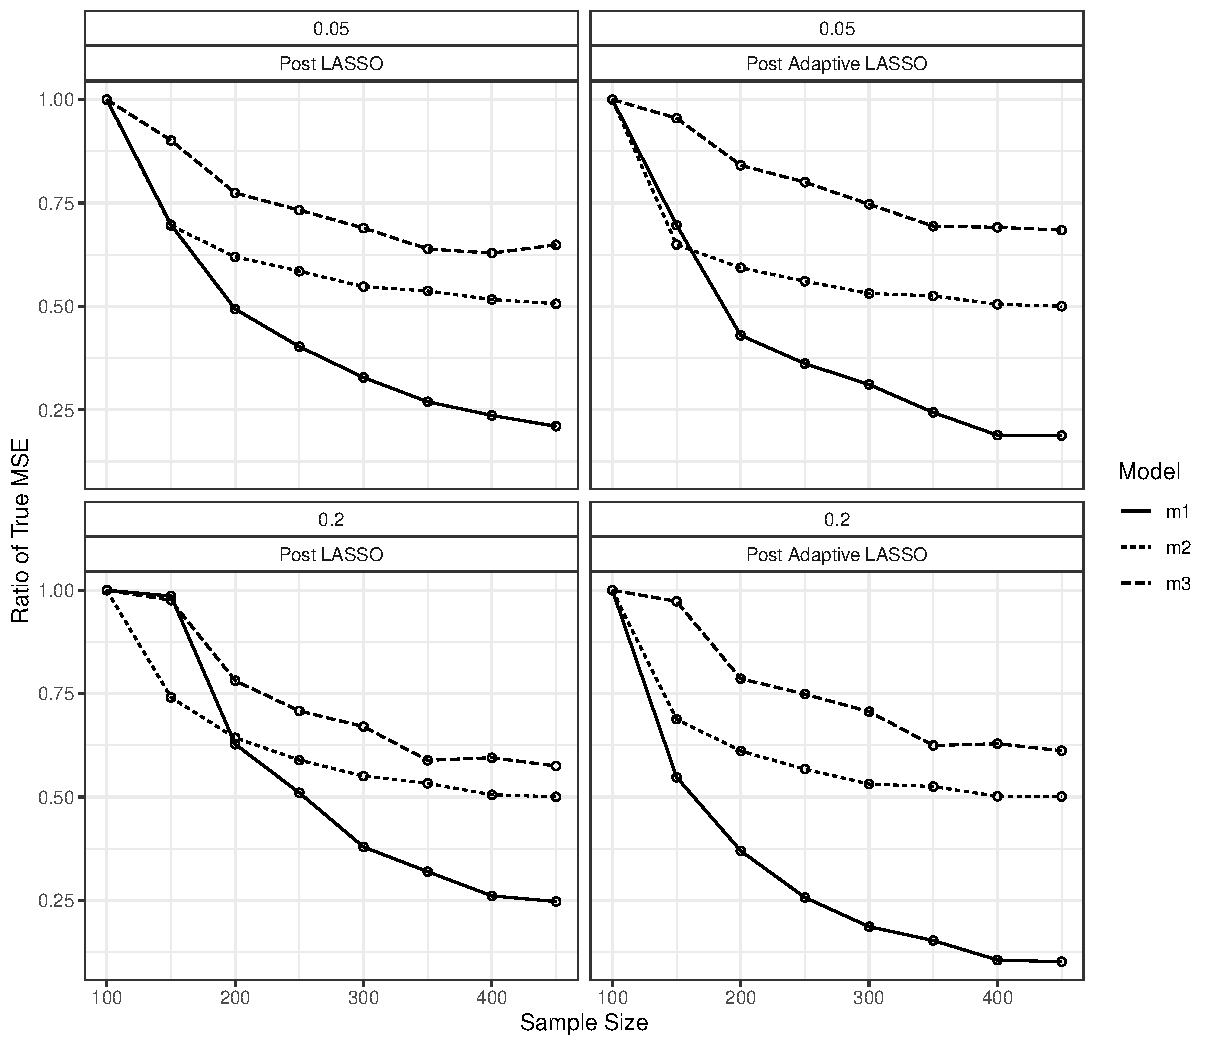
\includegraphics[width = 1.0\textwidth] {Graphics/rate.median.plot.pdf}
	%}
	\caption{Comparison of convergence rates (using median MSE)}
	\label{rate.median.plot}
    \end{figure}

        
		
		
	\clearpage
 
	\thispagestyle{empty}
	\section*{Versicherung an Eides statt}	
	
		\vspace{3cm}
		
		Ich versichere hiermit, dass ich die vorstehende Masterarbeit
		selbstständig verfasst und keine anderen als die angegebenen Quellen
		und Hilfsmittel benutzt habe, dass die vorgelegte Arbeit noch an keiner
		anderen Hochschule zur Prüfung vorgelegt wurde und dass sie weder
		ganz noch in Teilen bereits veröffentlicht wurde. Wörtliche Zitate und
		Stellen, die anderen Werken dem Sinn nach entnommen sind, habe ich
		in jedem einzelnen Fall kenntlich gemacht.
		
		\vspace{2cm}
		Bonn, 25.09.2023 \hrulefill \\
		\hspace*{0mm}Chencheng Fang
		
		\vspace{\fill}
\end{document}